%%%%%%%%%%%%%%%%%%%%%%%%%%%%%%%%%%%%%%%%%%%%%%%%%%%%%%%%%%%%%%%%%%%%%%
% Overleaf (WriteLaTeX) Example: Molecular Chemistry Presentation
%
% Source: http://www.overleaf.com
%
% In these slides we show how Overleaf can be used with standard 
% chemistry packages to easily create professional presentations.
% 
% Feel free to distribute this example, but please keep the referral
% to overleaf.com
% 
%%%%%%%%%%%%%%%%%%%%%%%%%%%%%%%%%%%%%%%%%%%%%%%%%%%%%%%%%%%%%%%%%%%%%%

\documentclass{beamer}

\mode<presentation>
{
  \usetheme{Madrid}       % or try default, Darmstadt, Warsaw, ...
  \usecolortheme{default} % or try albatross, beaver, crane, ...
  \usefonttheme{default}    % or try default, structurebold, ...
  \setbeamertemplate{navigation symbols}{}
  \setbeamertemplate{caption}[numbered]
} 

\usepackage[english]{babel}
\usepackage[utf8x]{inputenc}
\usepackage{graphicx}
\usepackage{hyperref}
  \hypersetup{colorlinks=true}
  \hypersetup{urlcolor=blue}
  \hypersetup{linkcolor = .}
\usepackage{xcolor}
\usepackage{siunitx}
  \sisetup{separate-uncertainty = true}
\usepackage{physics}
\usepackage[font=small,labelfont=bf]{caption}
\usepackage{subcaption}
\usepackage[en-GB]{datetime2}
\usepackage{overpic}
\usepackage{feynmp}
\DeclareGraphicsRule{*}{mps}{*}{}
\usepackage{scalerel}
\newcommand{\mylbrace}[2]{\vspace{#2pt}\hspace{6pt}\scaleleftright[\dimexpr5pt+#1\dimexpr0.06pt]{\lbrace}{\rule[\dimexpr2pt-#1\dimexpr0.5pt]{-4pt}{#1pt}}{.}}
\newcommand{\myrbrace}[2]{\vspace{#2pt}\scaleleftright[\dimexpr5pt+#1\dimexpr0.06pt]{.}{\rule[\dimexpr2pt-#1\dimexpr0.5pt]{-4pt}{#1pt}}{\rbrace}\hspace{6pt}}
\usepackage{ulem} % Line across text

% Here's where the presentation starts, with the info for the title slide
\title[$K^+K^-\pi^+\pi^-$]{\texorpdfstring{$D\to K^+K^-\pi^+\pi^-$}{K+K-pi+pi-} analysis at LHCb and BESIII}

\author{Martin Tat}
\institute{Oxford LHCb}
\date{30th May 2022}

\titlegraphic{
\includegraphics[height = 2cm]{lhcb.jpg}\hspace{1cm}~%
              
\includegraphics[height = 2cm]{OxfordLogo.pdf}\hspace{1cm}~%
              
\includegraphics[height = 2cm]{bes3.jpg}}

\begin{document}

\begin{frame}
  \titlepage
\end{frame}

% These three lines create an automatically generated table of contents.
\begin{frame}{Outline}
  \tableofcontents
\end{frame}

\section{LHCb}

\begin{frame}{$B^\pm\to(K^+K^-\pi^+\pi^-)_Dh^\pm$ GGSZ+GLW analysis at LHCb}
  \begin{center}
    {\huge $B^\pm\to(K^+K^-\pi^+\pi^-)_Dh^\pm$ \\~\\GGSZ+GLW analysis at LHCb}
  \end{center}
\end{frame}

\subsection{Summary of LHCb analysis status}

\begin{frame}{Summary of LHCb analysis status}
  \begin{itemize}
    \setlength\itemsep{0.5em}
    \item{Previously on $\gamma$ measurement in $B^\pm\to Dh^\pm$, $D\to K^+K^-\pi^+\pi^-$:}
    \begin{enumerate}
      \setlength\itemsep{0.5em}
      \item{Model-independent binned GGSZ and inclusive GLW analysis}
      \begin{itemize}
        \item{WG approval on 10th March}
        \item{Received 1st comments from RC reviewers, replies sent back}
      \end{itemize}
    \end{enumerate}
  \end{itemize}
  \begin{figure}
    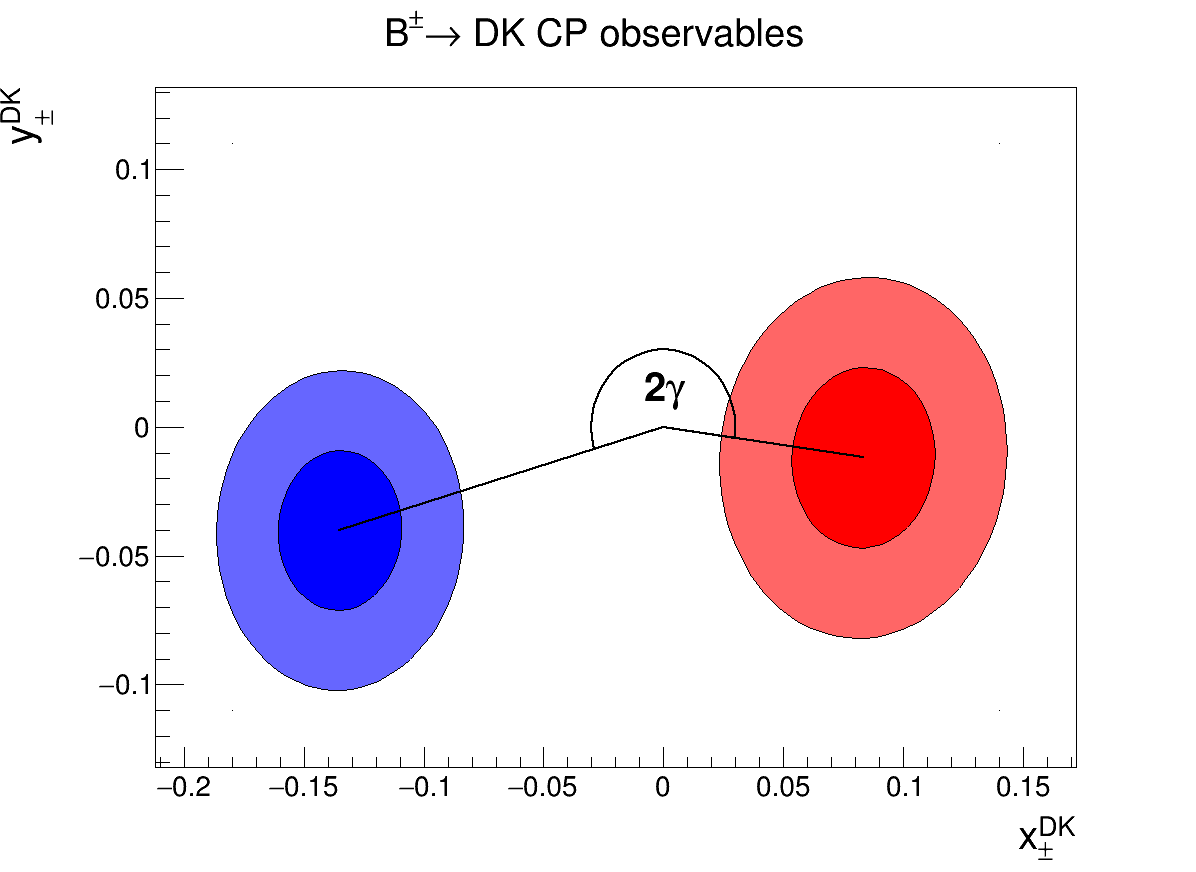
\includegraphics[width = 0.49\textwidth]{Plots/B2DK_CP_Observables_Contours.png}
    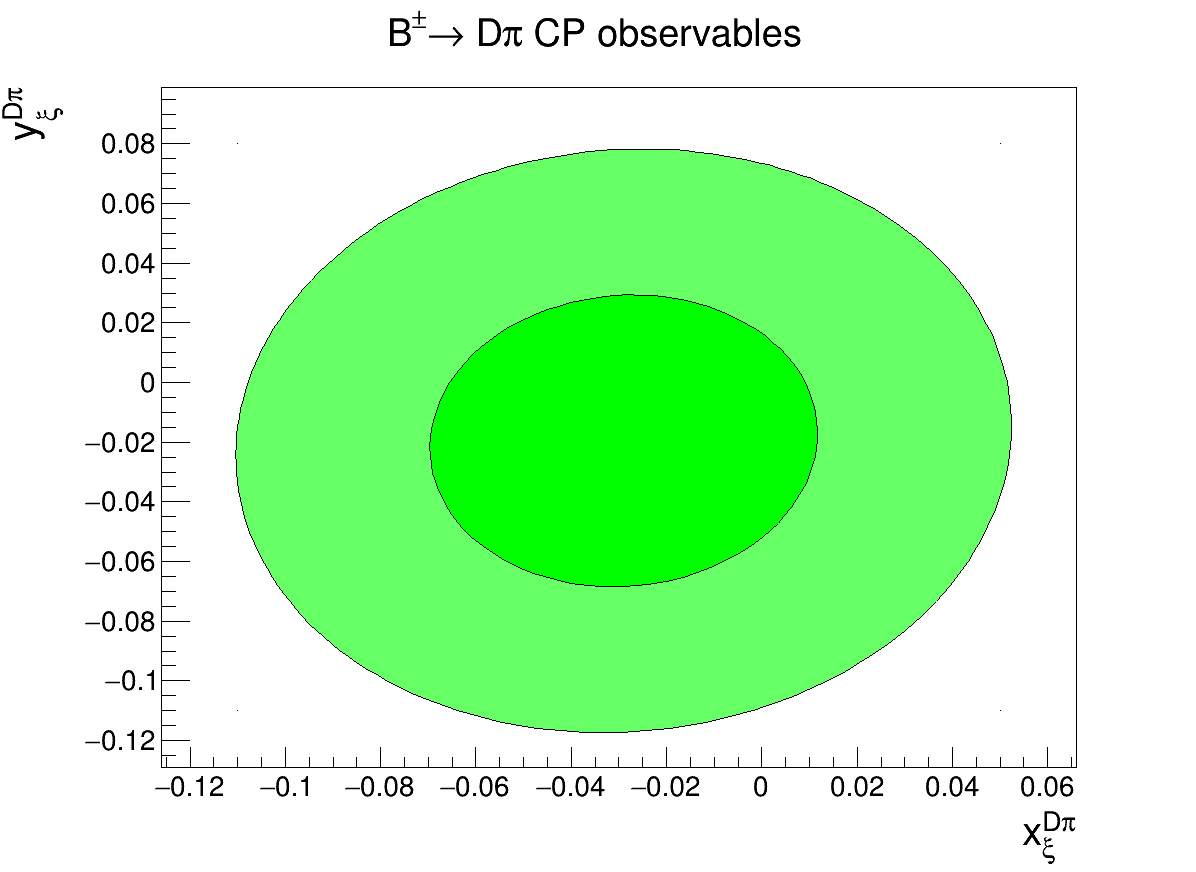
\includegraphics[width = 0.49\textwidth]{Plots/B2Dpi_CP_Observables_Contours.png}
  \end{figure}
\end{frame}

\begin{frame}{Results for $\gamma$}
  \vspace{-0.8cm}
  \begin{align*}
    \gamma =& \SI{103(14)}{\degree} \\
    \delta_B^{DK} =& \SI{92(14)}{\degree} \\
    r_B^{DK} =& \SI{0.117(20)}{} \\
    \delta_B^{D\pi} =& \SI{296(84)}{\degree} \\
    r_B^{D\pi} =& \SI{0.004(5)}{}
  \end{align*}
  \vspace{-0.8cm}
  \begin{itemize}
    \item{Sign error in the strong phase? $\gamma\to\SI{180}{\degree} - \gamma$}
    \item{Unfortunately, sign error looks unlikely...}
    \begin{itemize}
      \item{Interference fractions agree between LHCb and CLEO models}
      \item{BESIII data seems to support the sign from the model}
    \end{itemize}
  \end{itemize}
  \vspace{0.1cm}
  \begin{tabular}{l|c|c}
    Resonance                           & LHCb model phase ($\si{\radian}$) & CLEO model ($\si{\radian}$) \\
    \hline
    $D^0\to[\phi(1020)\rho^0]_{L = 0}$  & $0$ (fixed)                       & $0$ (fixed) \\
    $D^0\to K_1(1400)^+K^-$             & $1.05$                            & $-1.79$ \\
    $D^0\to K_1(1270)^+K^-$             & $2.02$                            & $-2.56$ \\
    \hline
  \end{tabular}
\end{frame}

\section{BESIII}

\begin{frame}{$D\to K^+K^-\pi^+\pi^-$ strong-phase analysis as BESIII}
  \begin{center}
    {\huge $D\to K^+K^-\pi^+\pi^-$ \\~\\strong-phase analysis as BESIII}
  \end{center}
\end{frame}

\subsection{Measurement of CP even fraction \texorpdfstring{$F_+$}{F+}}

\begin{frame}{Measurement of CP even fraction $F_+$}
  \begin{itemize}
    \item{BESIII: $e^+e^-$ collider at $\psi(3770)\to D^0\bar{D^0}$ threshold}
    \item{Reconstruct signal mode $D\to KK\pi\pi$ and a tag mode $D\to f$}
    \item{Signal mode is \underline{quantum correlated} with tag mode}
    \item{Measure BF with CP even/odd tags to determine $F_+$}
  \end{itemize}
  \begin{align*}
    \text{BF}(KK\pi\pi|f) =& \text{BF}(KK\pi\pi)\times\big(1 - \lambda_{\rm CP}(2F_+ - 1)\big) \\
    \text{BF}(KK\pi\pi|f) =& \text{BF}(KK\pi\pi)\times\big(K_i + K_{-i} \mp 2\sqrt{K_iK_{-i}}c_i(2F_+ - 1)\big)
  \end{align*}
  \begin{figure}[H]
    \centering
    \vspace{0.3cm}
    \begin{subfigure}{0.50\textwidth}
      \hspace{0.5cm}
      \begin{fmffile}{fgraph/fgraph_CPeven_tag}
        \setlength{\unitlength}{0.5cm}
        \begin{fmfgraph*}(8,4)
          \fmfstraight
          \fmfleft{i4,i3,i2,i1}
          \fmfright{g1,o1,o2,g2}
          \fmflabel{$K^+$}{o1}
          \fmflabel{$K^-$}{o2}
          \fmflabel{$K^+$}{i1}
          \fmflabel{$K^-$}{i2}
          \fmflabel{$\pi^+$}{i3}
          \fmflabel{$\pi^-$}{i4}
          \fmf{fermion}{w,i1}
          \fmf{fermion}{w,i2}
          \fmf{fermion}{w,i3}
          \fmf{fermion}{w,i4}
          \fmf{fermion}{w,o1}
          \fmf{fermion}{w,o2}
          \fmf{phantom}{w,g1}
          \fmf{phantom}{w,g2}
          \fmfblob{0.4cm}{w}
        \end{fmfgraph*}
      \end{fmffile}
      \vspace{0.3cm}
      \caption{CP even tag}
    \end{subfigure}%
    \begin{subfigure}{0.50\textwidth}
      \hspace{0.5cm}
      \begin{fmffile}{fgraph/fgraph_CPodd_tag}
        \setlength{\unitlength}{0.5cm}
        \begin{fmfgraph*}(8,4)
          \fmfstraight
          \fmfleft{i4,i3,i2,i1}
          \fmfright{g1,o1,o2,g2}
          \fmflabel{$\pi^0$}{o1}
          \fmflabel{$K_S$}{o2}
          \fmflabel{$K^+$}{i1}
          \fmflabel{$K^-$}{i2}
          \fmflabel{$\pi^+$}{i3}
          \fmflabel{$\pi^-$}{i4}
          \fmf{fermion}{w,i1}
          \fmf{fermion}{w,i2}
          \fmf{fermion}{w,i3}
          \fmf{fermion}{w,i4}
          \fmf{fermion}{w,o1}
          \fmf{fermion}{w,o2}
          \fmf{phantom}{w,g1}
          \fmf{phantom}{w,g2}
          \fmfblob{0.4cm}{w}
        \end{fmfgraph*}
      \end{fmffile}
      \vspace{0.3cm}
      \caption{CP odd tag}
    \end{subfigure}
    \vspace{0.0cm}
  \end{figure}
\end{frame}

\begin{frame}{$F_+$ measurement with CP, $K^0_S\pi^+\pi^-$ and $K^0_L\pi^+\pi^-$ tags}
  \begin{figure}
    \begin{subfigure}{0.40\textwidth}
      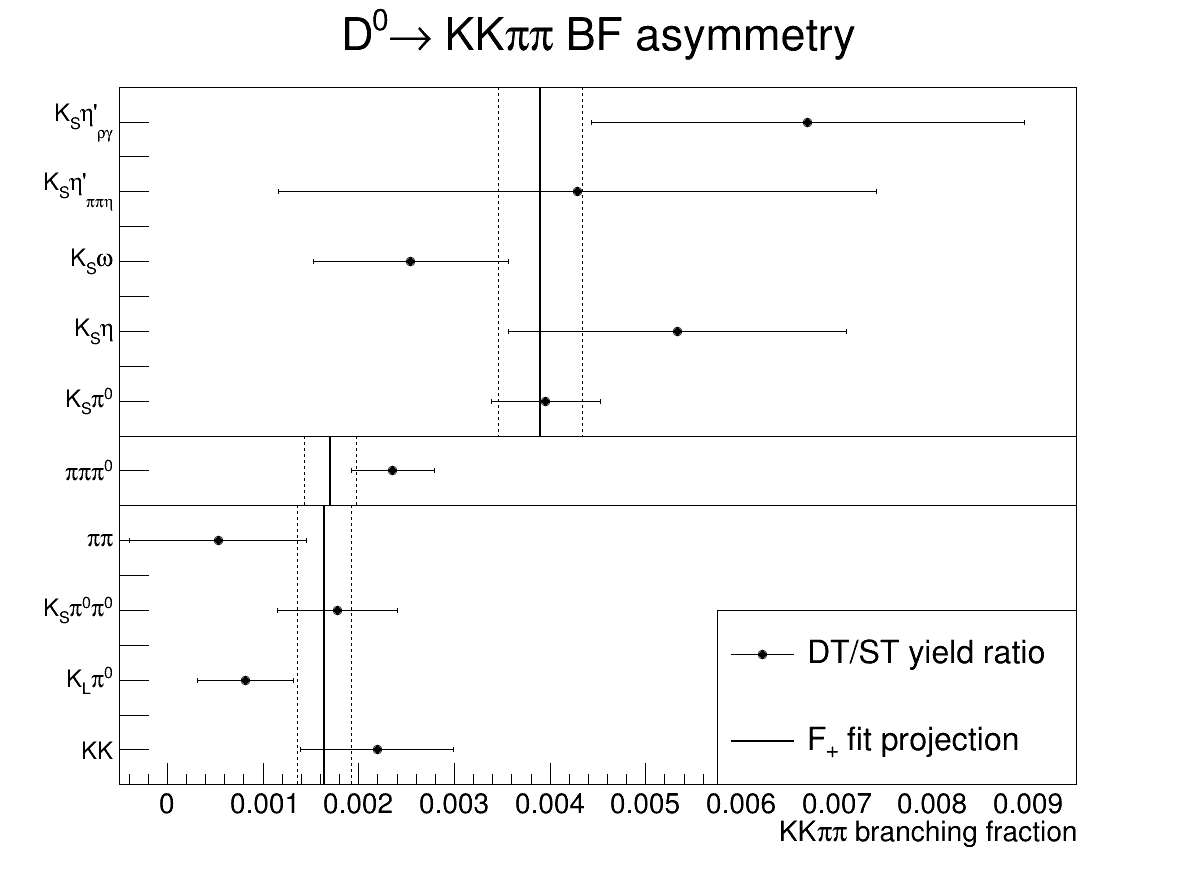
\includegraphics[width = 1.0\textwidth]{Plots/CPeven_fraction_combination_CPtags.png}
      \caption{CP tags}
    \end{subfigure}
    \begin{subfigure}{0.35\textwidth}
      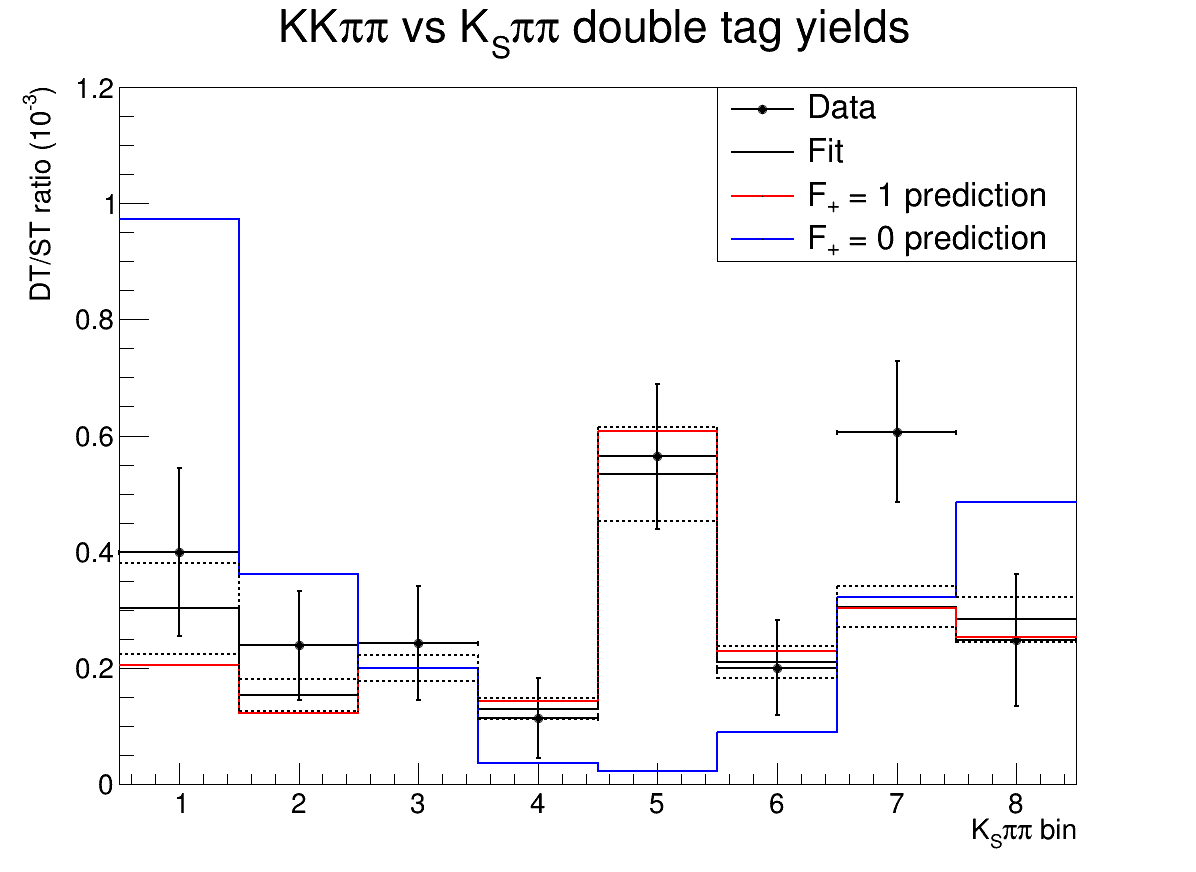
\includegraphics[width = 1.0\textwidth]{Plots/CPeven_fraction_combination_KSpipi.png}
      \caption{$K^0_S\pi^+\pi^-$ tag}
    \end{subfigure}%
    \begin{subfigure}{0.35\textwidth}
      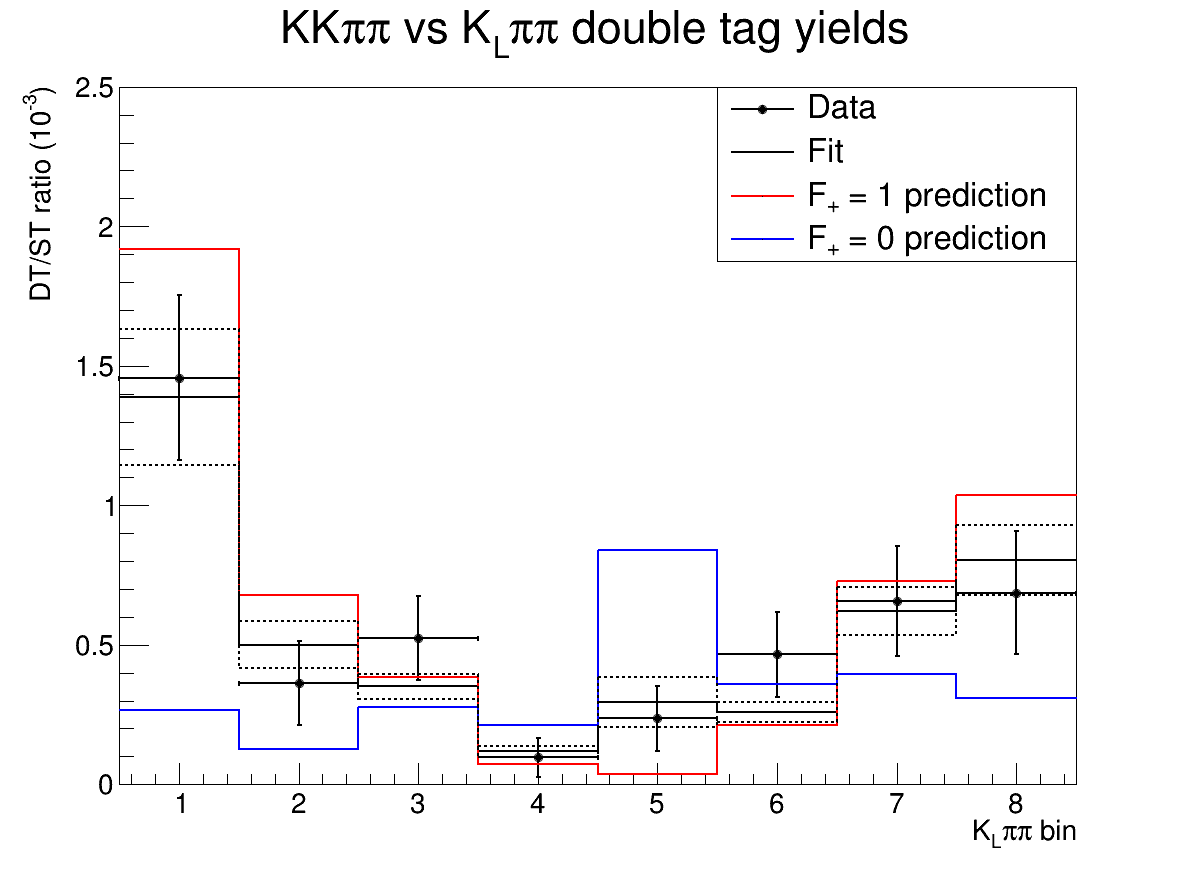
\includegraphics[width = 1.0\textwidth]{Plots/CPeven_fraction_combination_KLpipi.png}
      \caption{$K^0_L\pi^+\pi^-$ tag}
    \end{subfigure}
  \end{figure}
\end{frame}

\begin{frame}{$F_+$ combination}
  \begin{figure}
    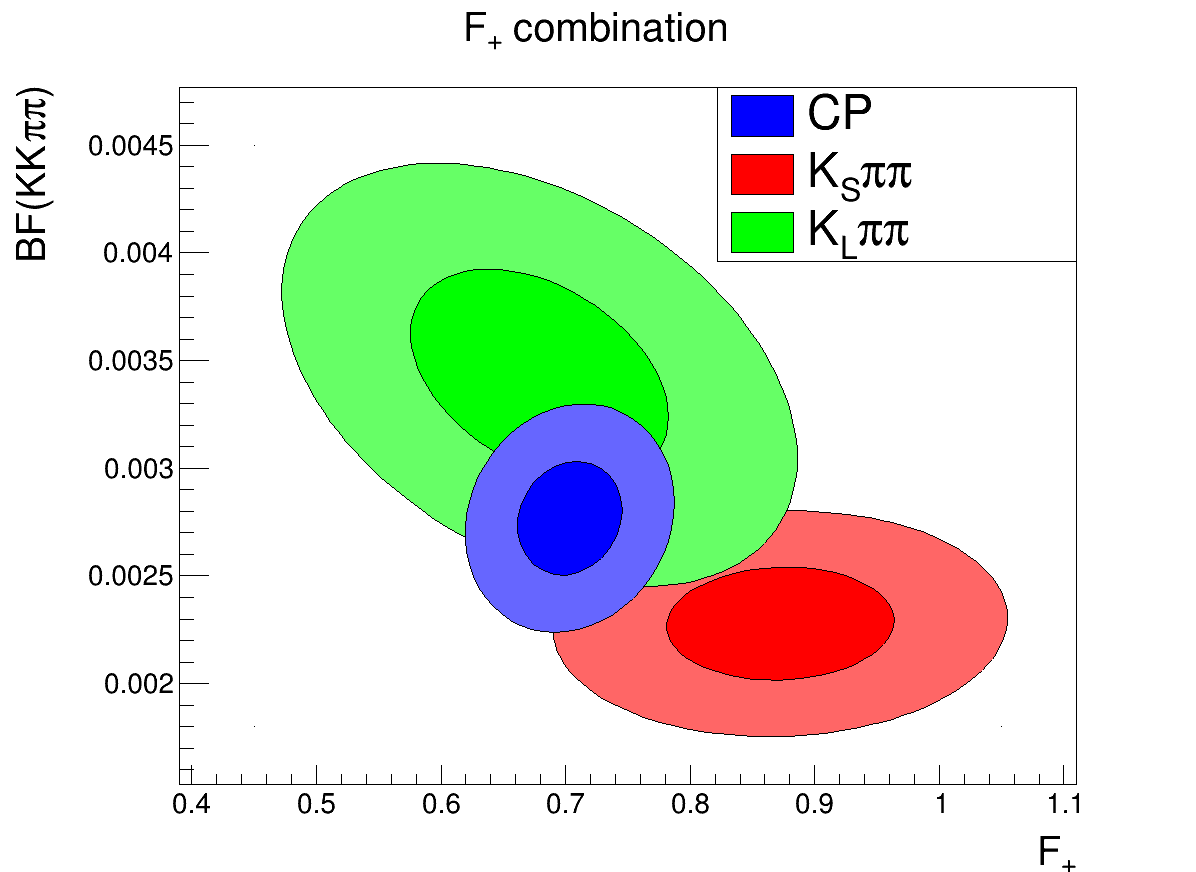
\includegraphics[width = 0.55\textwidth]{Plots/FPlus_contours.png}
    \caption{$F_+$ combination}
  \end{figure}
  \vspace{-0.6cm}
  \begin{itemize}
    \item{Observe large anti-correlation in $K_L\pi\pi$ because $F^{K_L\pi\pi}_+\approx 0.354$}
    \begin{itemize}
      \item{Yield of $K_L\pi\pi$ is \underline{twice} as large as that of $K_S\pi\pi$}
      \item{Fractional bin yields \underline{and} total yield contains information about $F_+$}
      \item{When $K_L\pi\pi$ BF is available, combine all tags!}
    \end{itemize}
  \end{itemize}
\end{frame}

\subsection{Efficiency corrections}

\begin{frame}{Efficiency corrections}
  \begin{itemize}
    \setlength\itemsep{1.5em}
    \item{All yields must be corrected for efficiency}
    \item{Problem: BESIII simulation uses a very old $KK\pi\pi$ model in EvtGen}
    \item{Solution: Reweight BESIII simulation to look like the LHCb model}
    \begin{itemize}
      \setlength\itemsep{0.5em}
      \item{Use Python hep\textunderscore ml Gradient Boosted Reweighter}
      \item{Variables:}
      \begin{enumerate}
        \item{$m^2(K^+K^-)$}
        \item{$m^2(K^+\pi^-)$}
        \item{$m^2(K^-\pi^+)$}
        \item{$m^2(\pi^+\pi^-)$}
        \item{$m^2(K^+K^-\pi^+)$}
      \end{enumerate}
    \end{itemize}
  \end{itemize}
\end{frame}

\begin{frame}{Naive efficiency correction}
  \begin{figure}
    \begin{subfigure}{0.33\textwidth}
      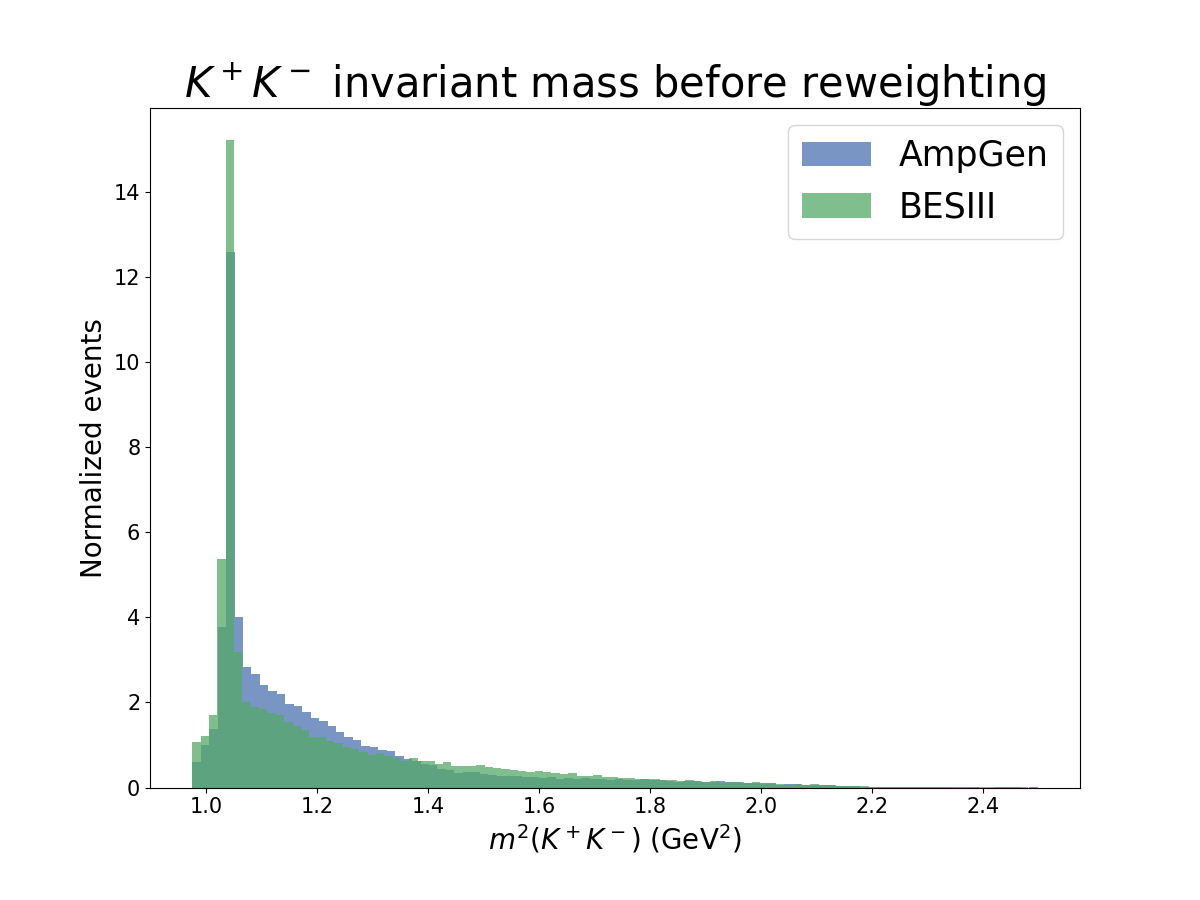
\includegraphics[width = 1.0\textwidth]{Plots/s01_BeforeReweighting.png}
      \caption{$m^2(K^+K^-)$}
    \end{subfigure}%
    \begin{subfigure}{0.33\textwidth}
      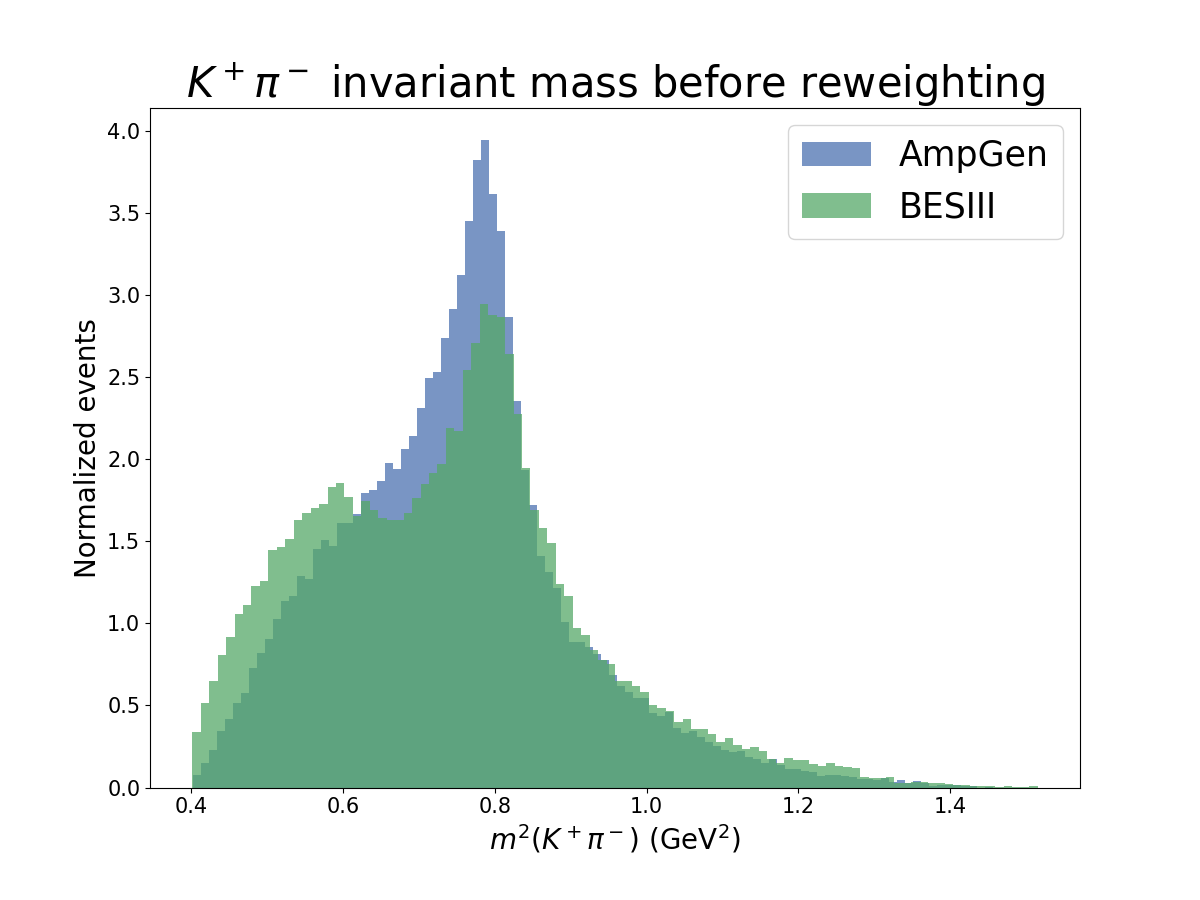
\includegraphics[width = 1.0\textwidth]{Plots/s03_BeforeReweighting.png}
      \caption{$m^2(K^+\pi^-)$}
    \end{subfigure}%
    \begin{subfigure}{0.33\textwidth}
      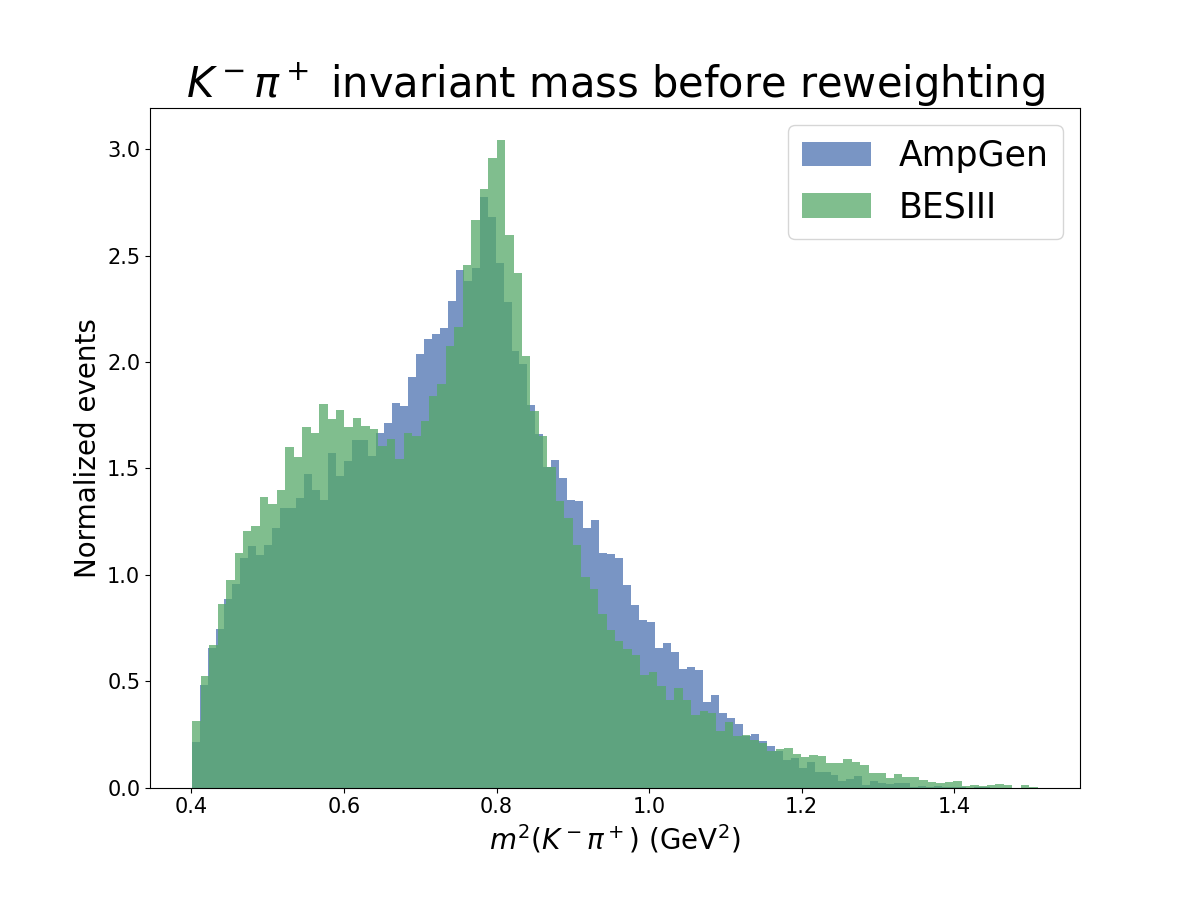
\includegraphics[width = 1.0\textwidth]{Plots/s12_BeforeReweighting.png}
      \caption{$m^2(K^-\pi^+)$}
    \end{subfigure}
    \begin{subfigure}{0.33\textwidth}
      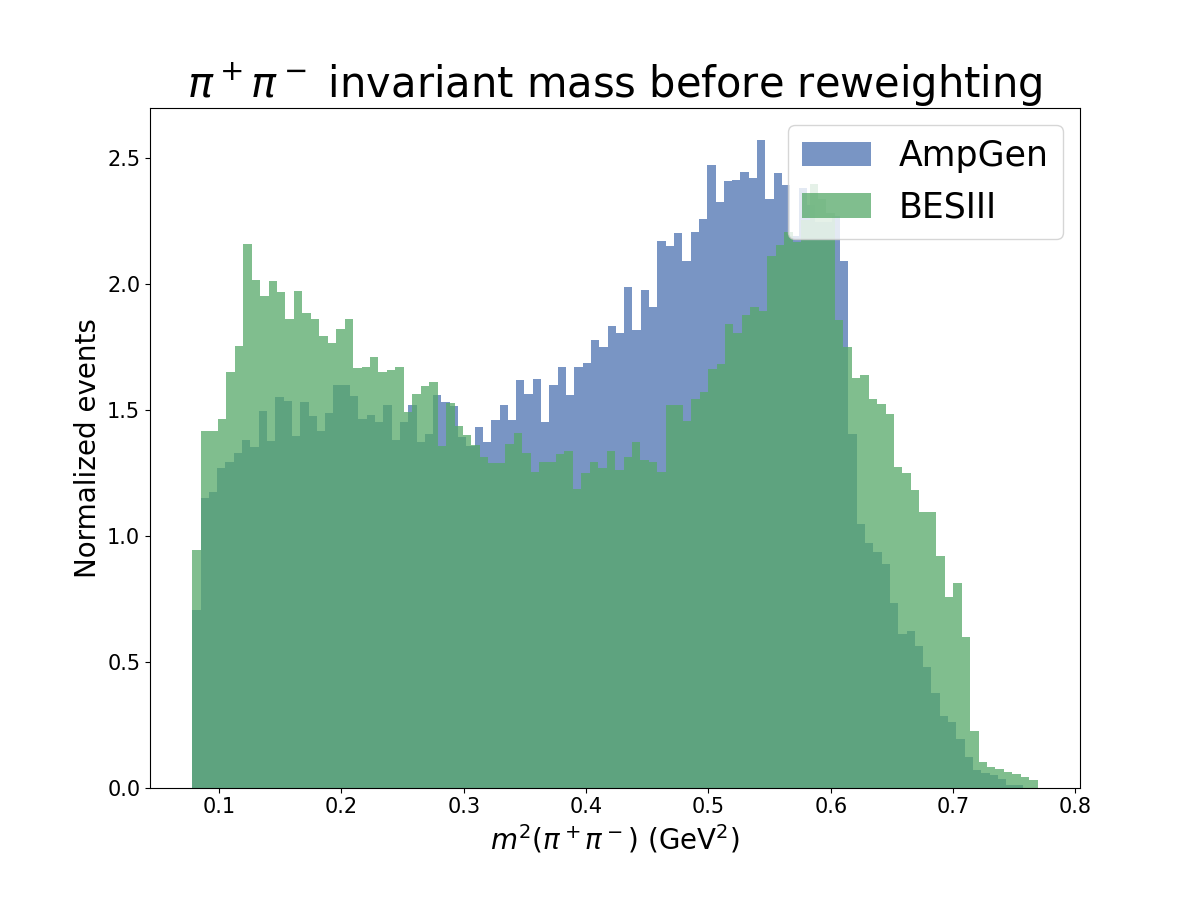
\includegraphics[width = 1.0\textwidth]{Plots/s23_BeforeReweighting.png}
      \caption{$m^2(\pi^+\pi^-)$}
    \end{subfigure}%
    \begin{subfigure}{0.33\textwidth}
      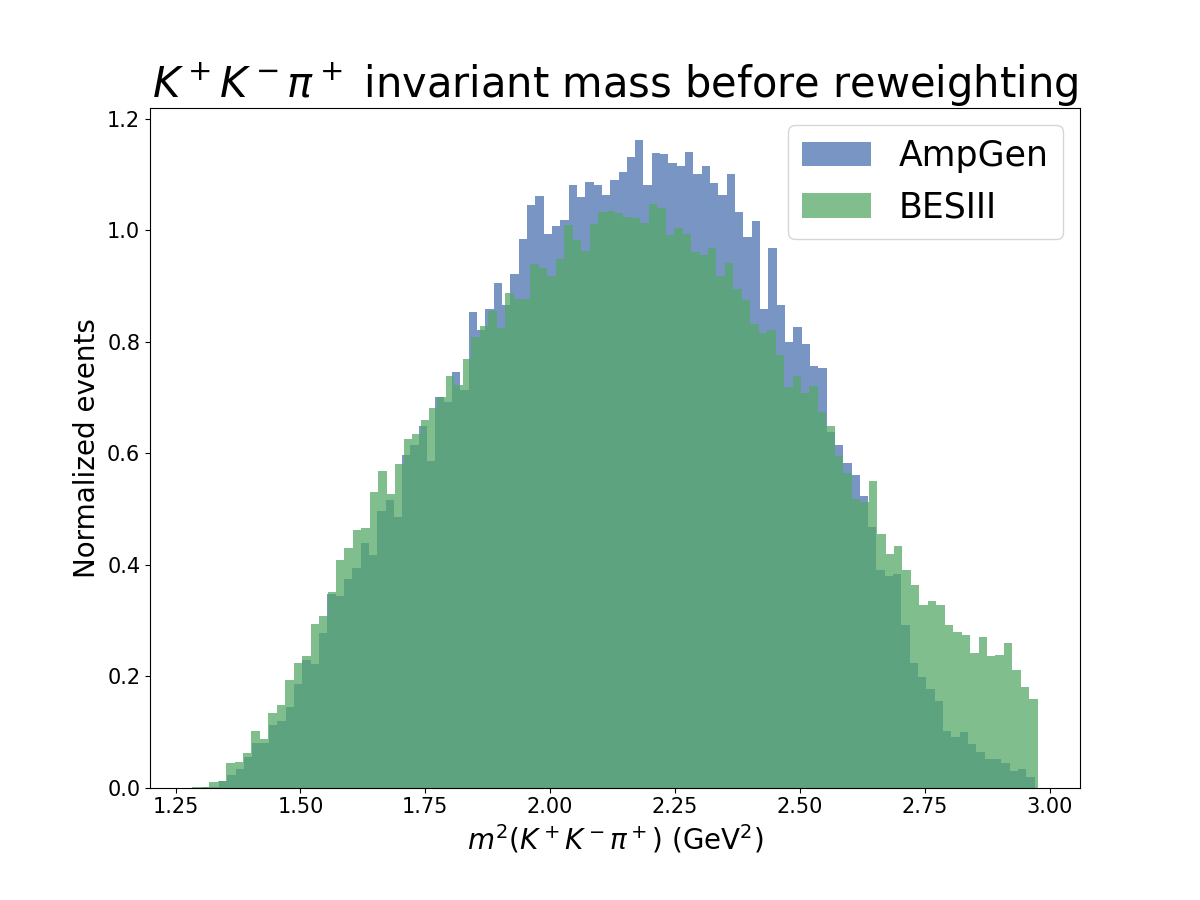
\includegraphics[width = 1.0\textwidth]{Plots/s012_BeforeReweighting.png}
      \caption{$m^2(K^+K^-\pi^+)$}
    \end{subfigure}
    \caption{Before reweighting}
  \end{figure}
\end{frame}

\begin{frame}{Naive efficiency correction}
  \begin{figure}
    \begin{subfigure}{0.33\textwidth}
      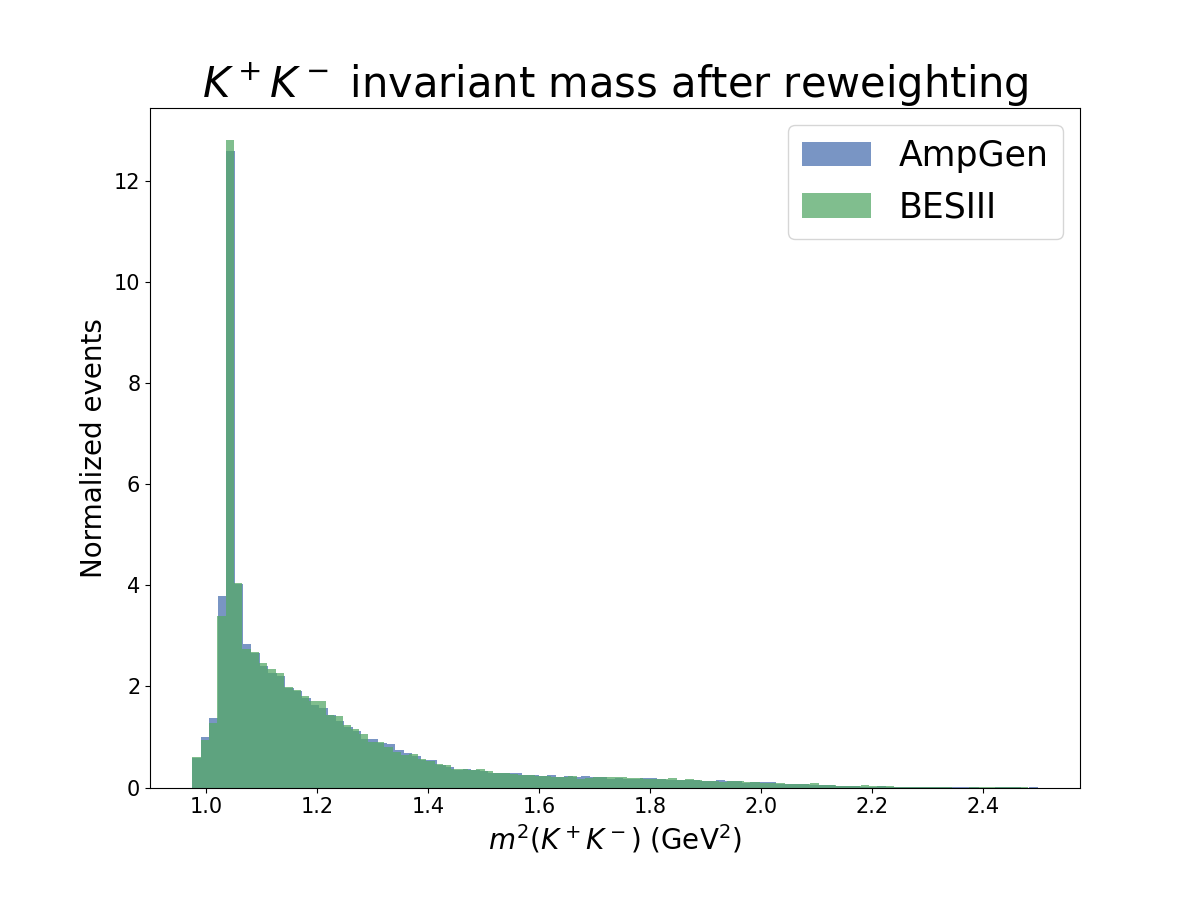
\includegraphics[width = 1.0\textwidth]{Plots/s01_AfterReweighting.png}
      \caption{$m^2(K^+K^-)$}
    \end{subfigure}%
    \begin{subfigure}{0.33\textwidth}
      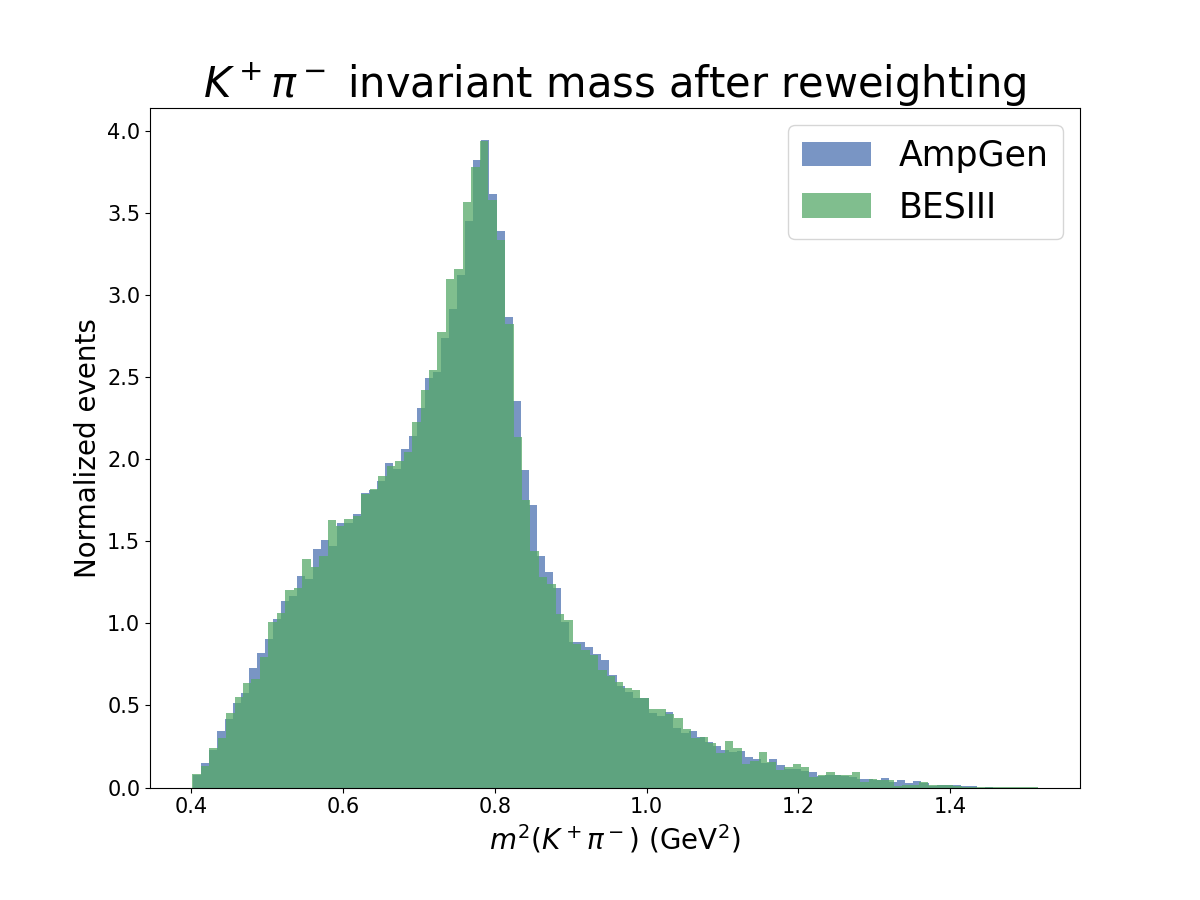
\includegraphics[width = 1.0\textwidth]{Plots/s03_AfterReweighting.png}
      \caption{$m^2(K^+\pi^-)$}
    \end{subfigure}%
    \begin{subfigure}{0.33\textwidth}
      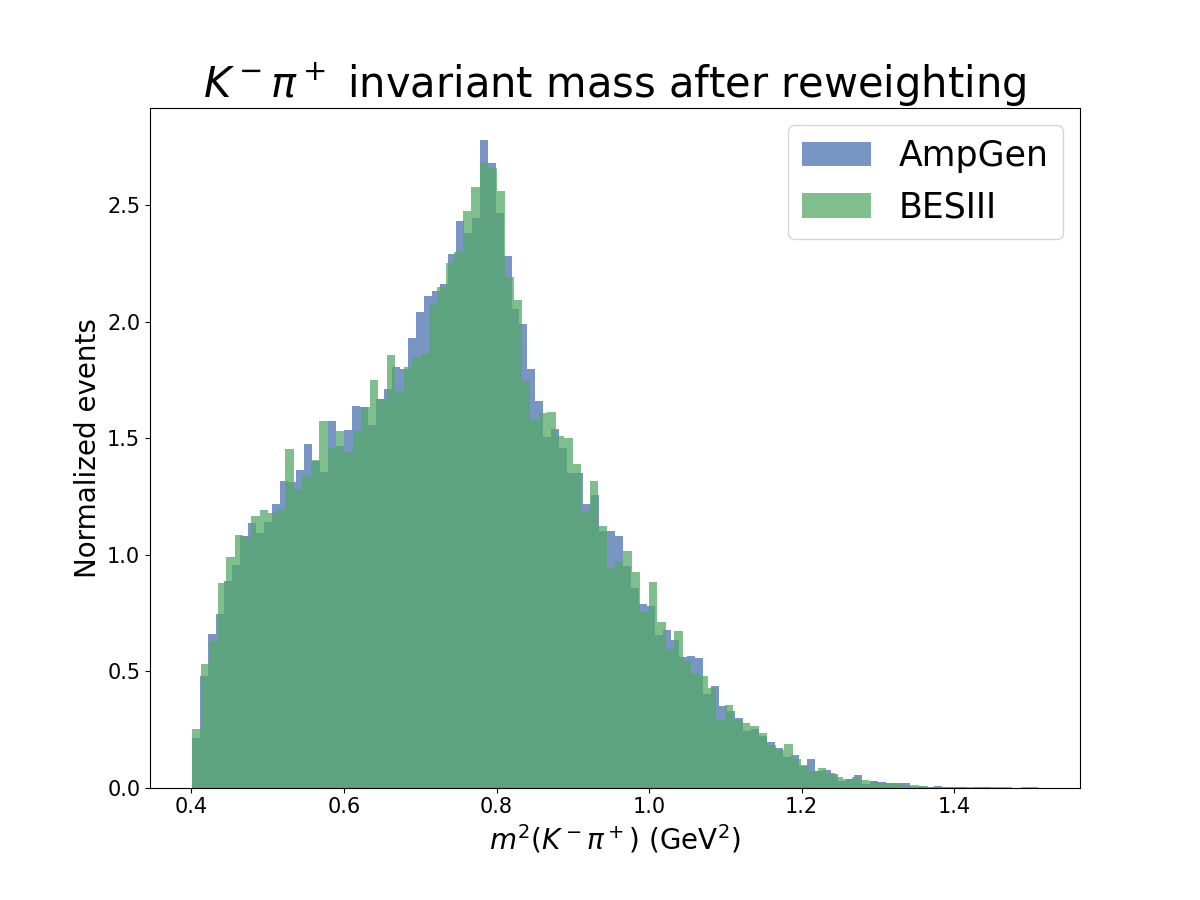
\includegraphics[width = 1.0\textwidth]{Plots/s12_AfterReweighting.png}
      \caption{$m^2(K^-\pi^+)$}
    \end{subfigure}
    \begin{subfigure}{0.33\textwidth}
      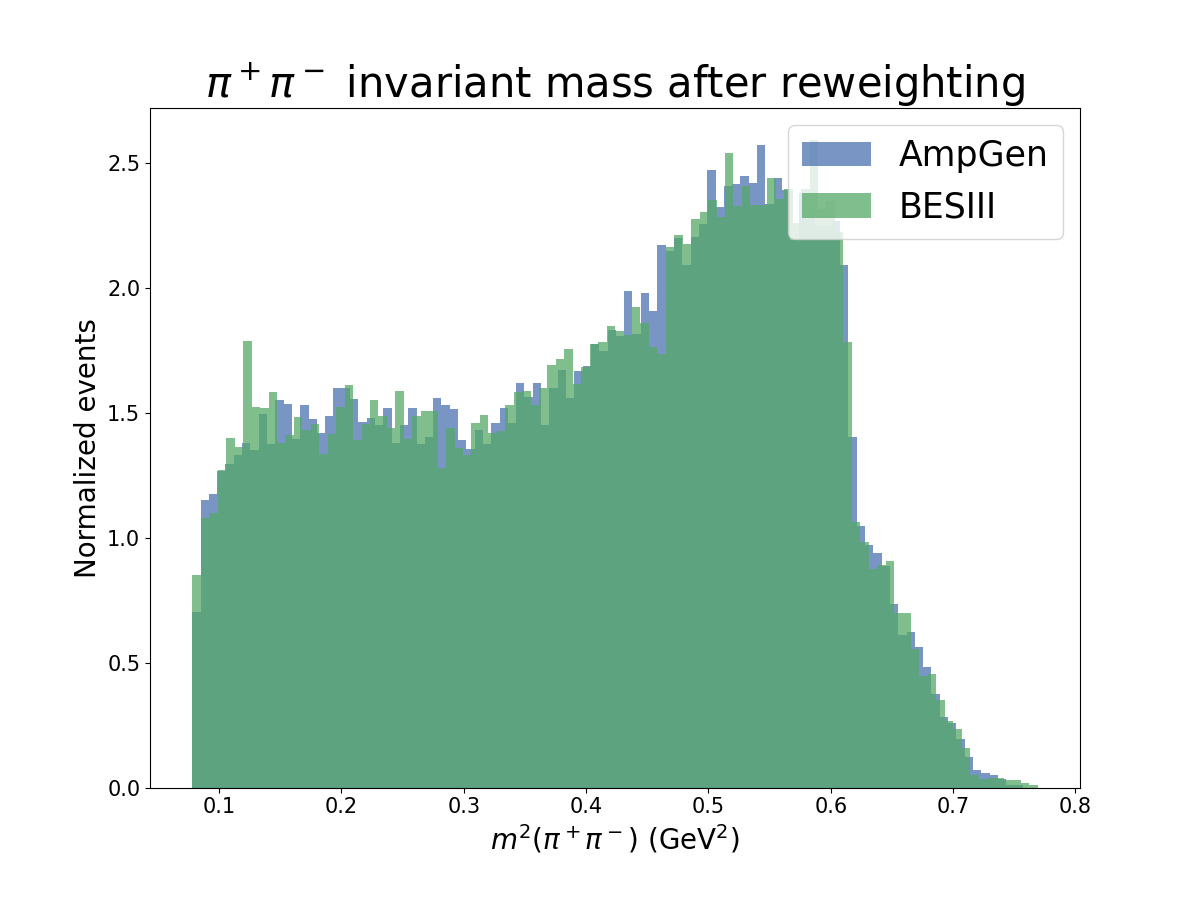
\includegraphics[width = 1.0\textwidth]{Plots/s23_AfterReweighting.png}
      \caption{$m^2(\pi^+\pi^-)$}
    \end{subfigure}%
    \begin{subfigure}{0.33\textwidth}
      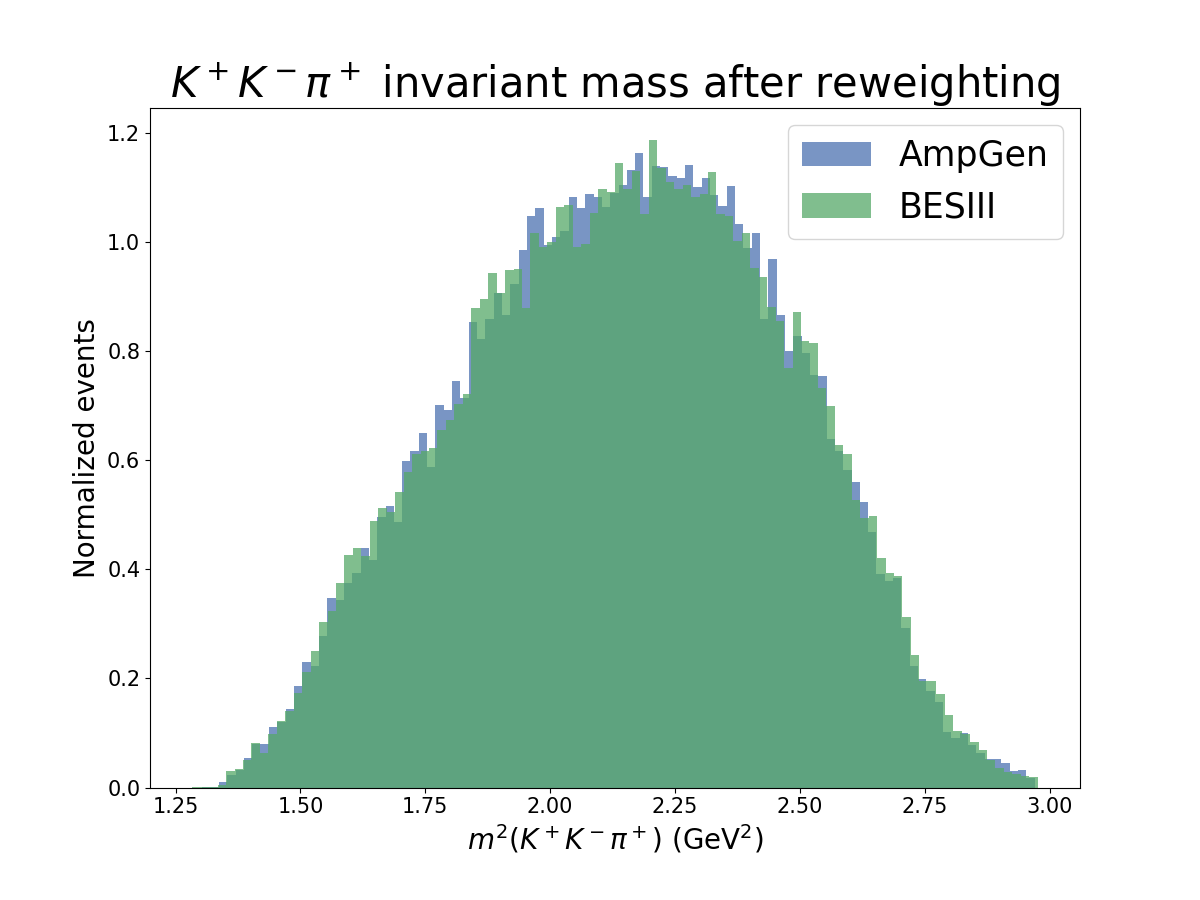
\includegraphics[width = 1.0\textwidth]{Plots/s012_AfterReweighting.png}
      \caption{$m^2(K^+K^-\pi^+)$}
    \end{subfigure}
    \caption{After reweighting}
  \end{figure}
\end{frame}

\begin{frame}{Does the naive reweighting work?}
  \begin{figure}
    \begin{subfigure}{0.33\textwidth}
      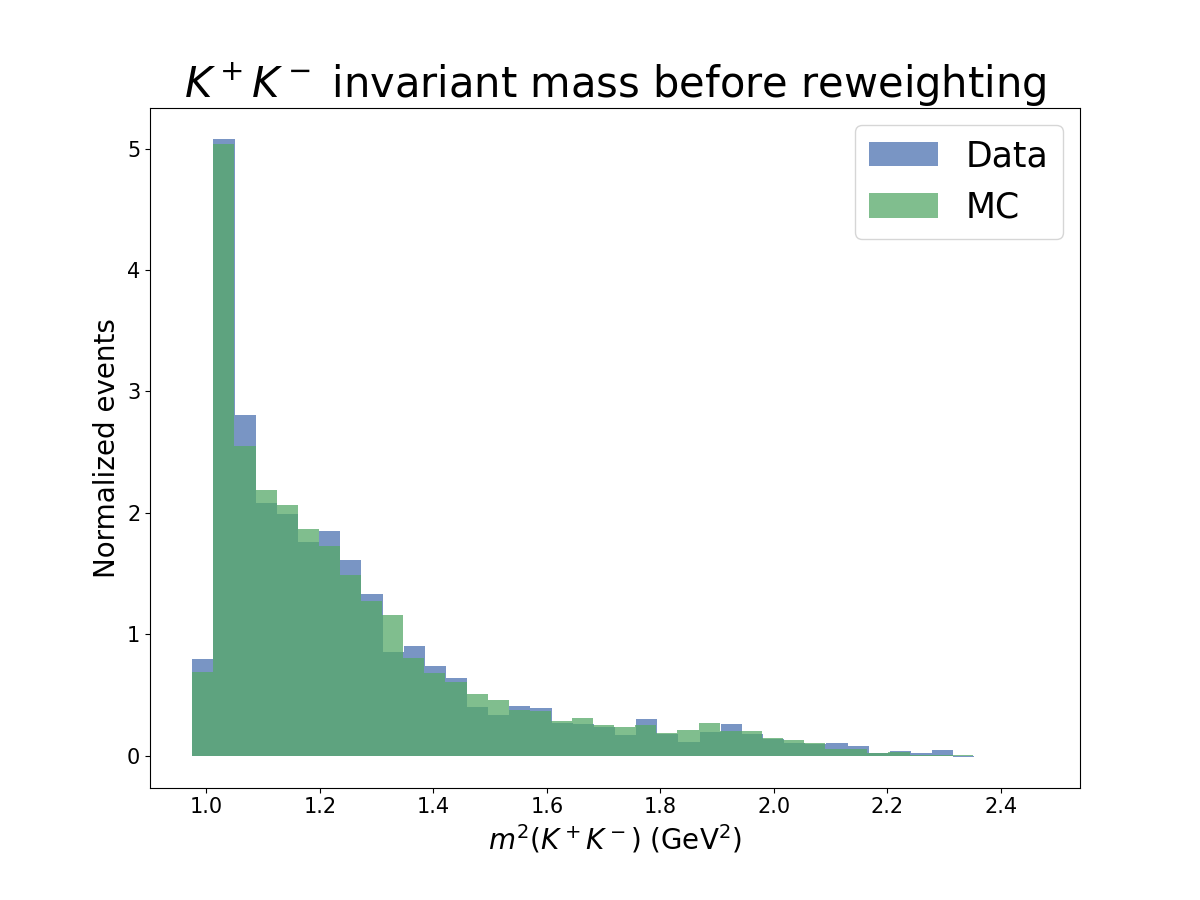
\includegraphics[width = 1.0\textwidth]{Plots/s01_DataMCMismatch_BeforeReweighting.png}
      \caption{$m^2(K^+K^-)$}
    \end{subfigure}%
    \begin{subfigure}{0.33\textwidth}
      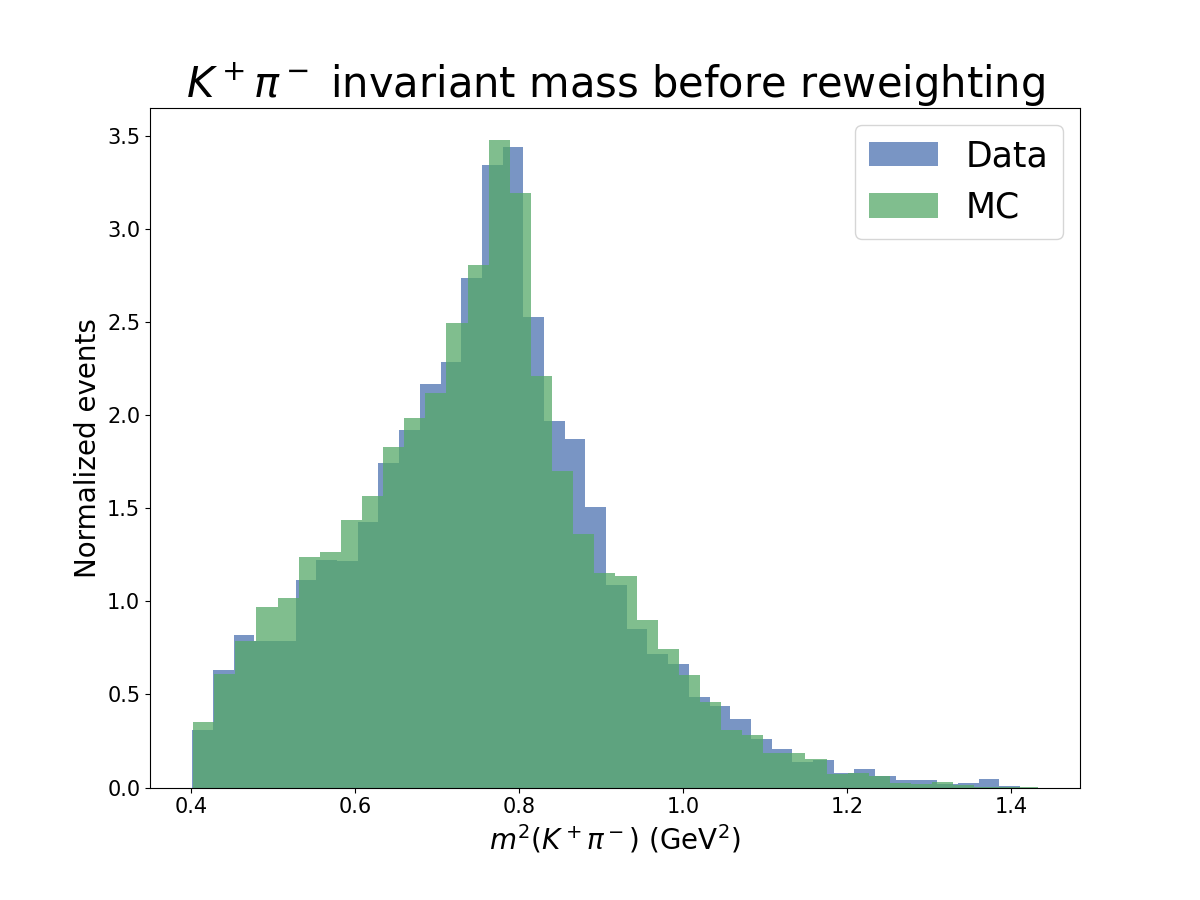
\includegraphics[width = 1.0\textwidth]{Plots/s03_DataMCMismatch_BeforeReweighting.png}
      \caption{$m^2(K^+\pi^-)$}
    \end{subfigure}%
    \begin{subfigure}{0.33\textwidth}
      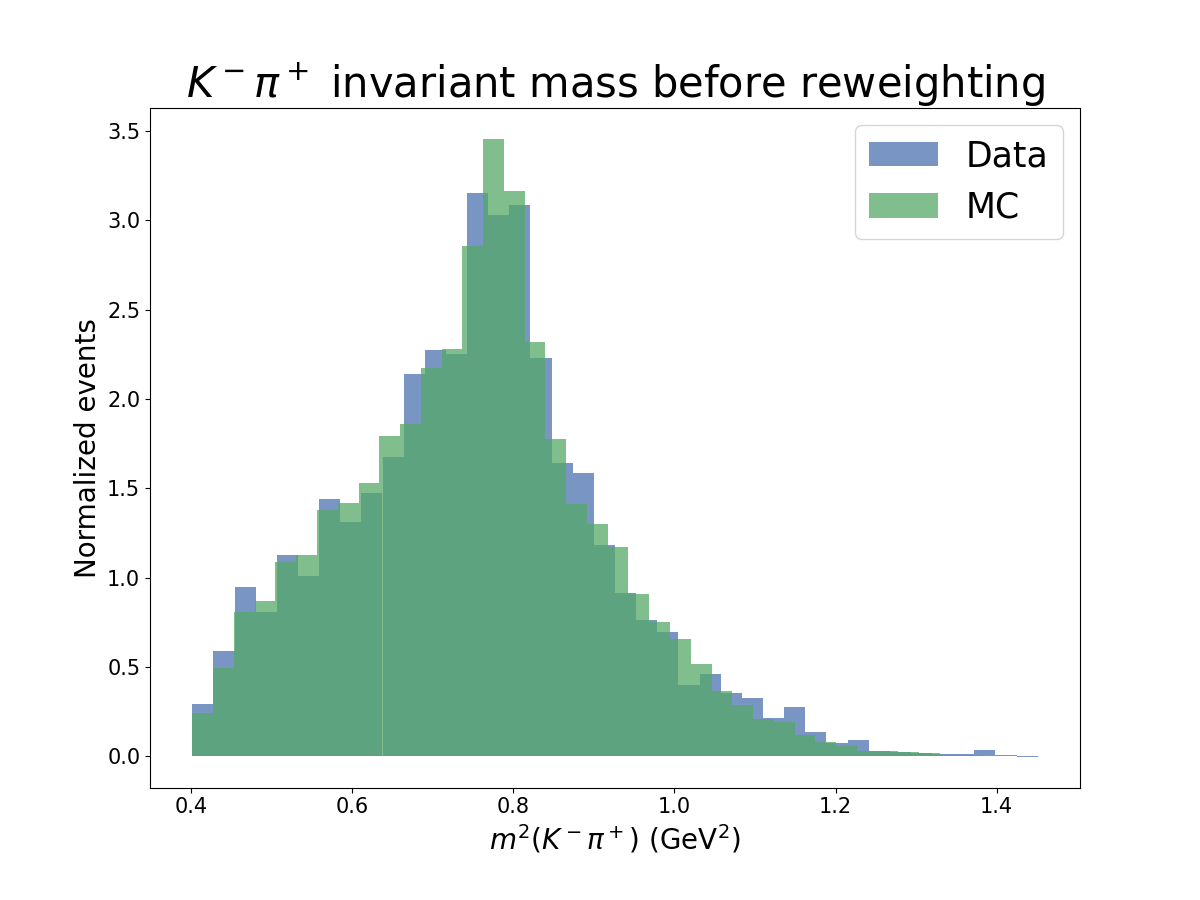
\includegraphics[width = 1.0\textwidth]{Plots/s12_DataMCMismatch_BeforeReweighting.png}
      \caption{$m^2(K^-\pi^+)$}
    \end{subfigure}
    \begin{subfigure}{0.33\textwidth}
      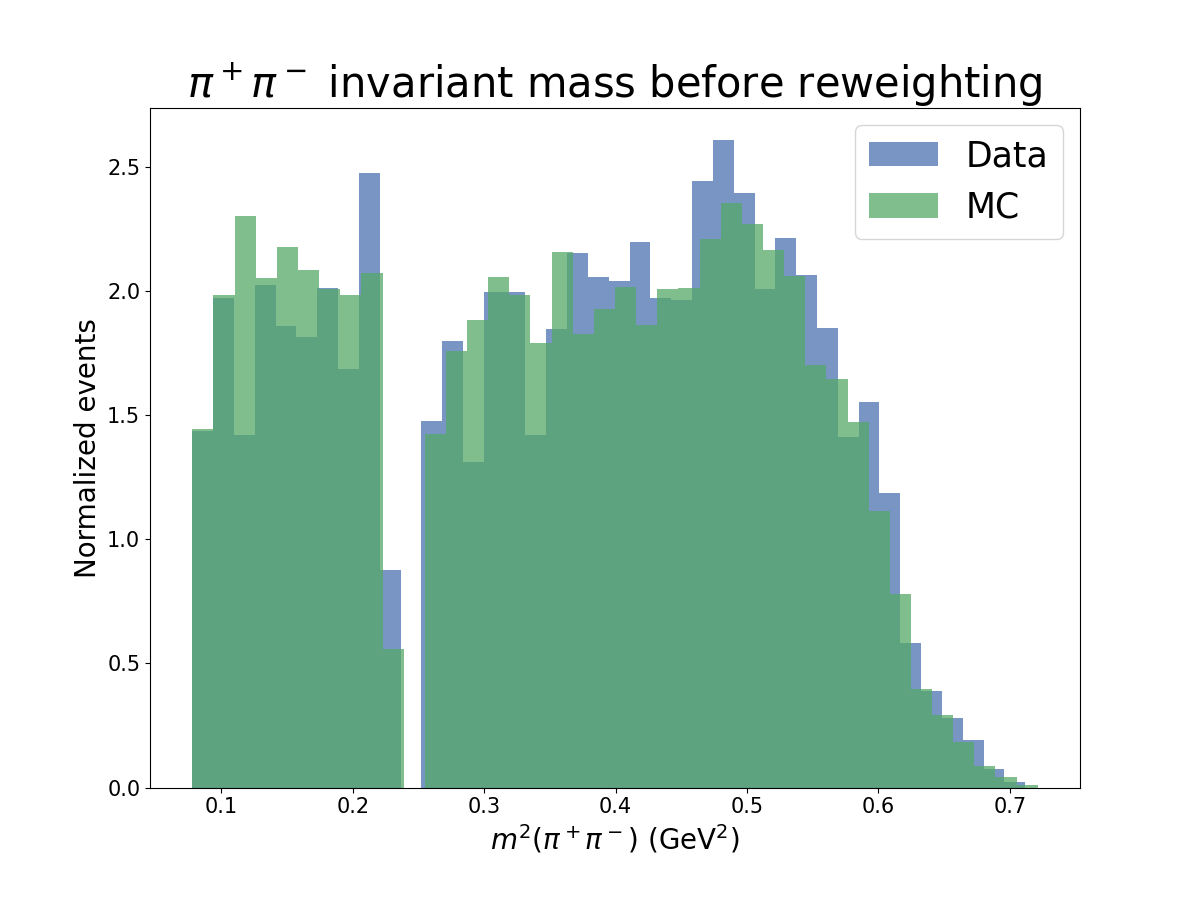
\includegraphics[width = 1.0\textwidth]{Plots/s23_DataMCMismatch_BeforeReweighting.png}
      \caption{$m^2(\pi^+\pi^-)$}
    \end{subfigure}%
    \begin{subfigure}{0.33\textwidth}
      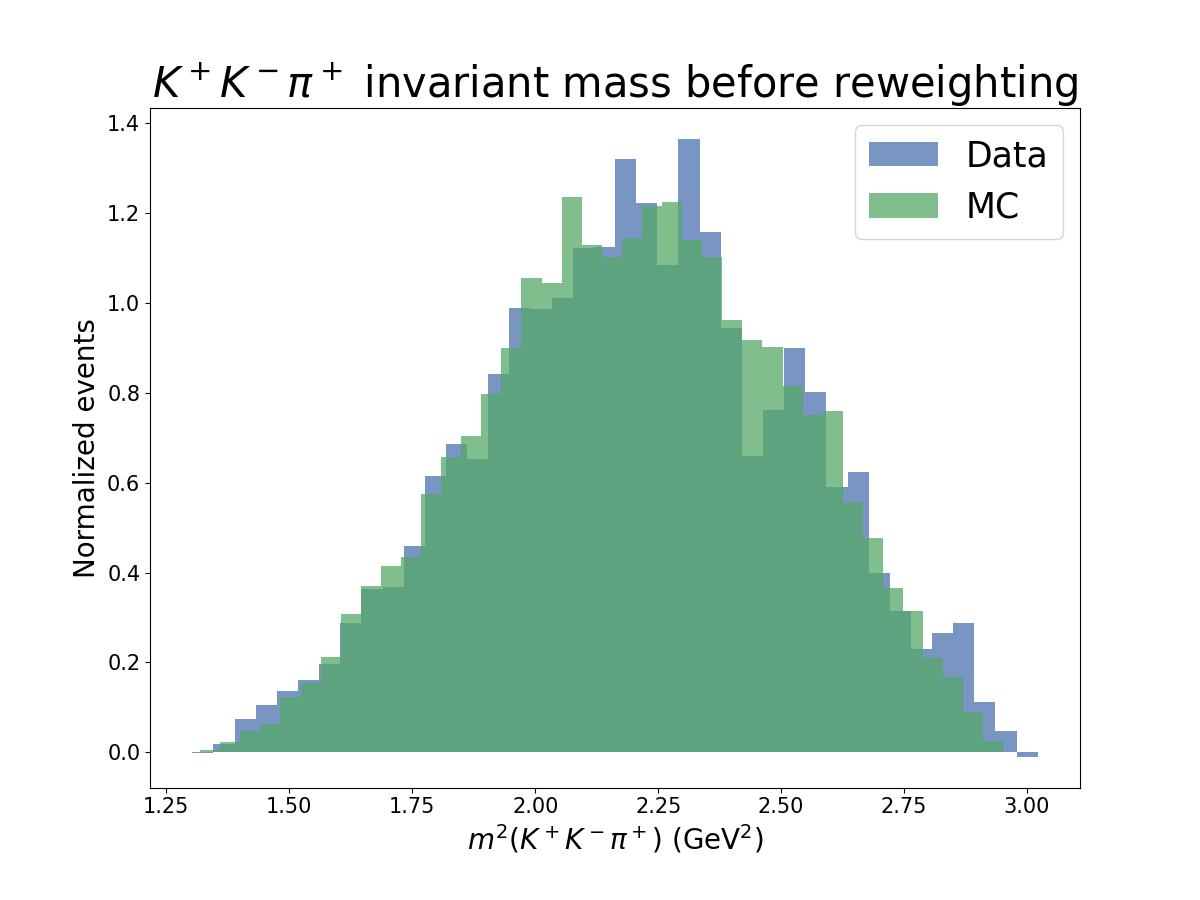
\includegraphics[width = 1.0\textwidth]{Plots/s012_DataMCMismatch_BeforeReweighting.png}
      \caption{$m^2(K^+K^-\pi^+)$}
    \end{subfigure}
    \caption{Single tag $D\to KK\pi\pi$ in data and MC after reweighting}
  \end{figure}
\end{frame}

\begin{frame}{Quantum correlated LHCb model}
  \begin{itemize}
    \setlength\itemsep{1.5em}
    \item{Problem with naive reweighting:}
    \begin{itemize}
    \setlength\itemsep{1.0em}
      \item{LHCb model assumes a pure $D^0\to K^+K^-\pi^+\pi^-$ decay}
      \item{\underline{No} quantum correlations}
      \item{Example: If tag is $D\to KK$, the $D\to KK\pi\pi$ decay will be CP odd!}
      \item{Quantum correlations will affect phase space distribution $\implies$ Efficiencies could change}
    \end{itemize}
    \item{Solution: Separate reweighters for CP even/odd $D\to K^+K^-\pi^+\pi^-$}
    \begin{itemize}
    \setlength\itemsep{1.0em}
      \item{CP even tags: Use efficiencies after reweighting to CP odd model}
      \item{CP odd tags: Use efficiencies after reweighting to CP even model}
      \item{$K_{S, L}\pi\pi$ tags: Do a weighted average of the two efficiencies}
    \end{itemize}
  \end{itemize}
\end{frame}

\begin{frame}{Before weighting to CP even/odd models}
  \begin{figure}
    \begin{subfigure}{0.50\textwidth}
      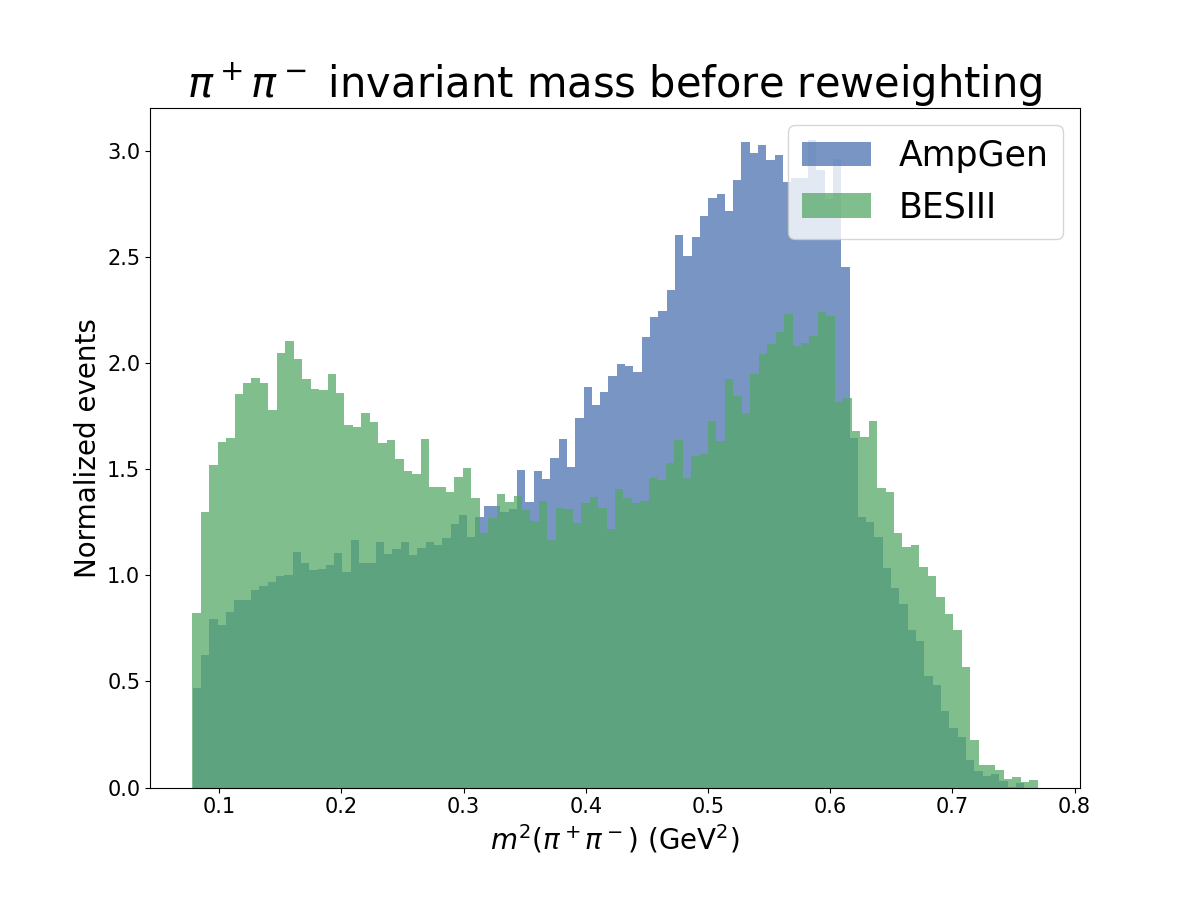
\includegraphics[width = 1.0\textwidth]{Plots/s23_BeforeReweighting_CPEven.png}
      \caption{CP even}
    \end{subfigure}%
    \begin{subfigure}{0.50\textwidth}
      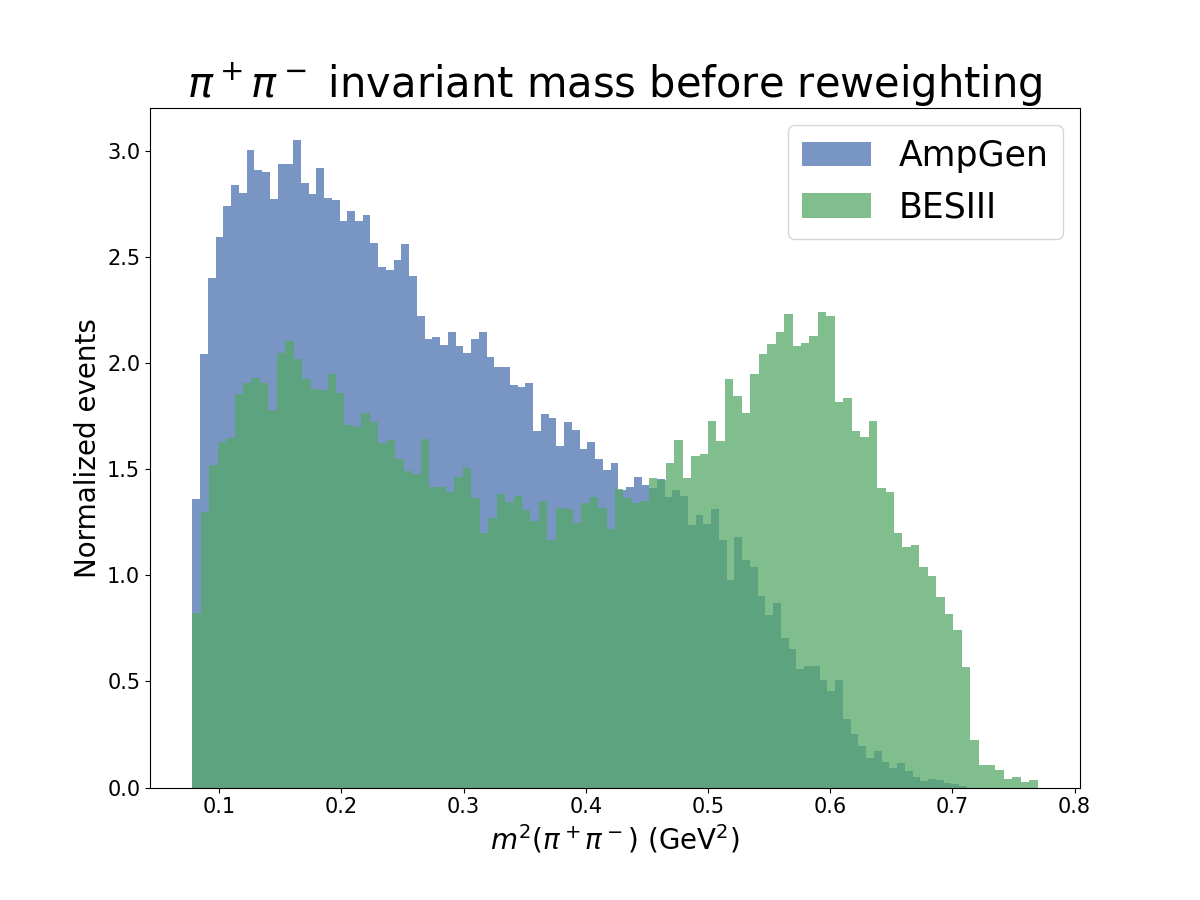
\includegraphics[width = 1.0\textwidth]{Plots/s23_BeforeReweighting_CPOdd.png}
      \caption{CP odd}
    \end{subfigure}
    \caption{$m^2(\pi^+\pi^-)$ before reweighting}
  \end{figure}
\end{frame}

\begin{frame}{After weighting to CP even/odd models}
  \begin{figure}
    \begin{subfigure}{0.50\textwidth}
      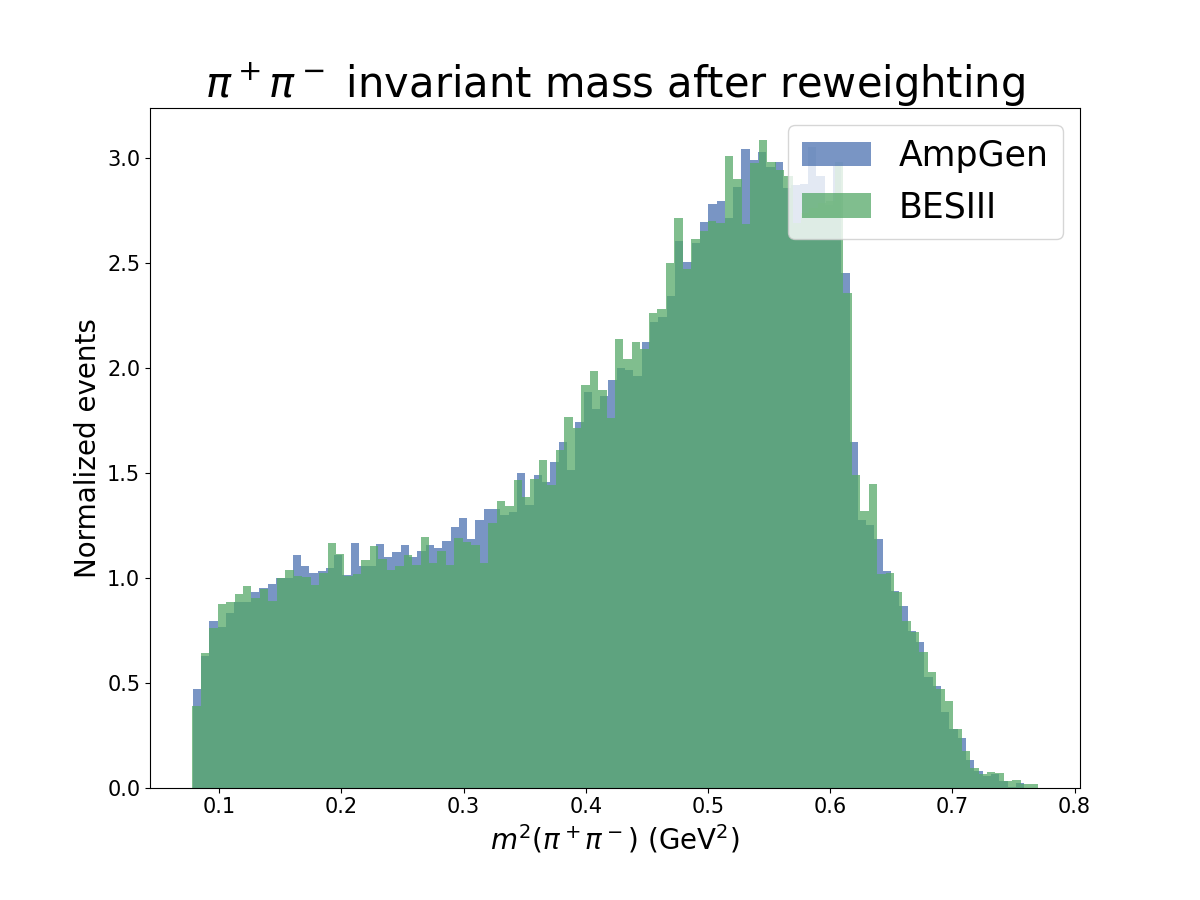
\includegraphics[width = 1.0\textwidth]{Plots/s23_AfterReweighting_CPEven.png}
      \caption{CP even}
    \end{subfigure}%
    \begin{subfigure}{0.50\textwidth}
      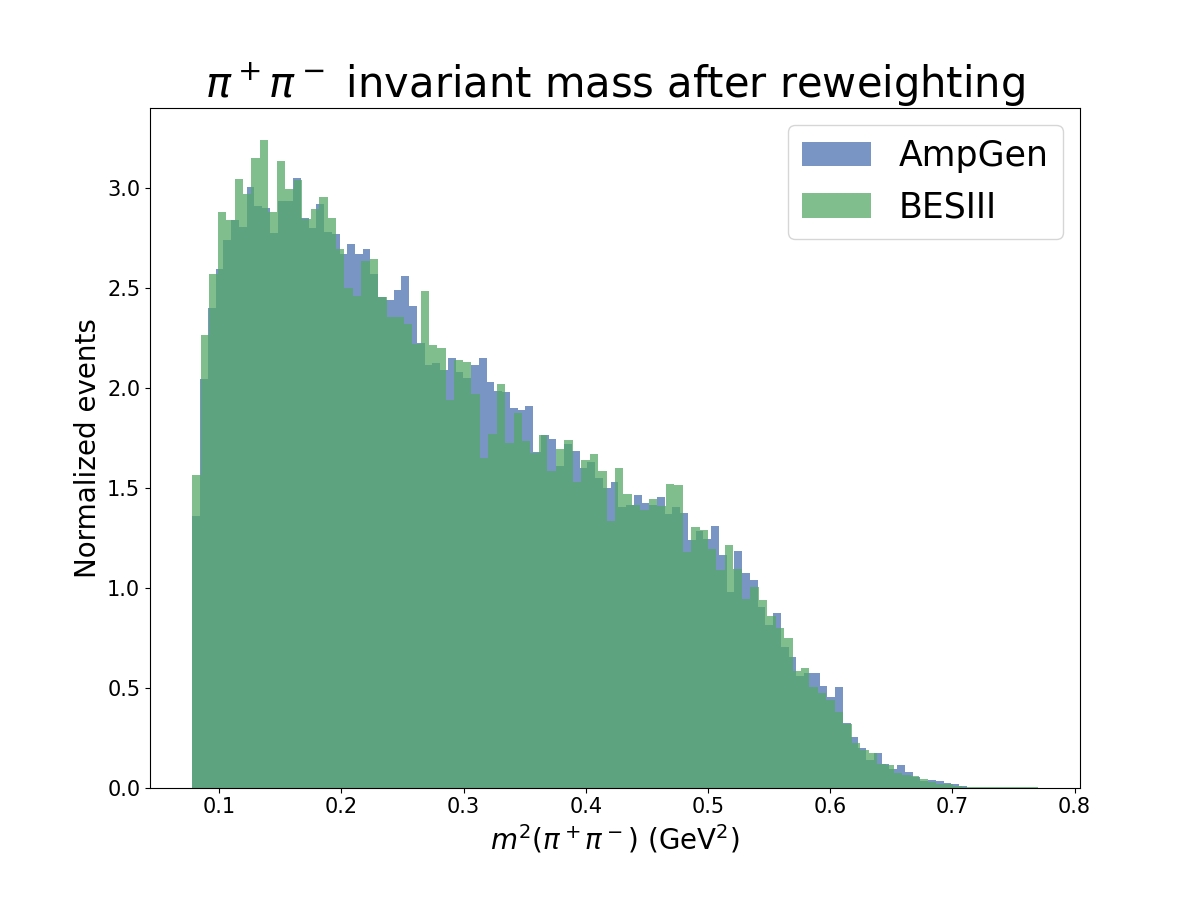
\includegraphics[width = 1.0\textwidth]{Plots/s23_AfterReweighting_CPOdd.png}
      \caption{CP odd}
    \end{subfigure}
    \caption{$m^2(\pi^+\pi^-)$ after reweighting}
  \end{figure}
  \vspace{-0.4cm}
  \begin{tabular}{cccc}
    \hline
    No reweighting & Naive reweighting & CP even model & CP odd model \\
    \hline
    $18.0\%$       & $19.0\%$          & $18.1\%$      & $21.9\%$ \\
    \hline
  \end{tabular}
\end{frame}

\begin{frame}{Agreement between quantum correlated data and model}
  \begin{itemize}
    \item{Note: LHCb model knows \underline{nothing} about quantum correlations}
    \item{$D^0$/$\bar{D^0}$ amplitudes simply combined to obtain CP even/odd models}
    \item{Important question: Can the model describe quantum correlated double tag data at all? Answer: Yes!}
  \end{itemize}
  \begin{figure}
    \begin{subfigure}{0.50\textwidth}
      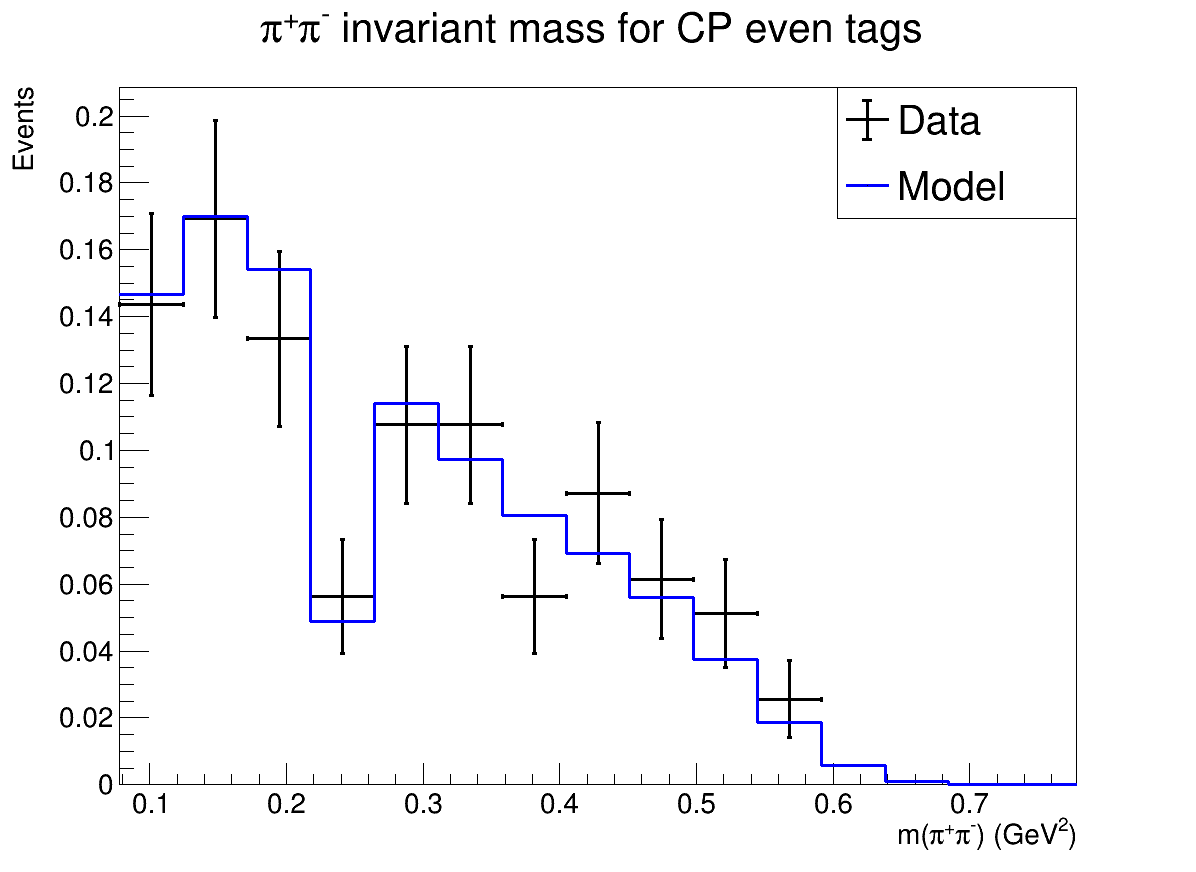
\includegraphics[width = 1.0\textwidth]{Plots/s23_DataModel_CPEvenTags.png}
      \caption{Double tags of $KK\pi\pi$ vs CP even}
    \end{subfigure}%
    \begin{subfigure}{0.50\textwidth}
      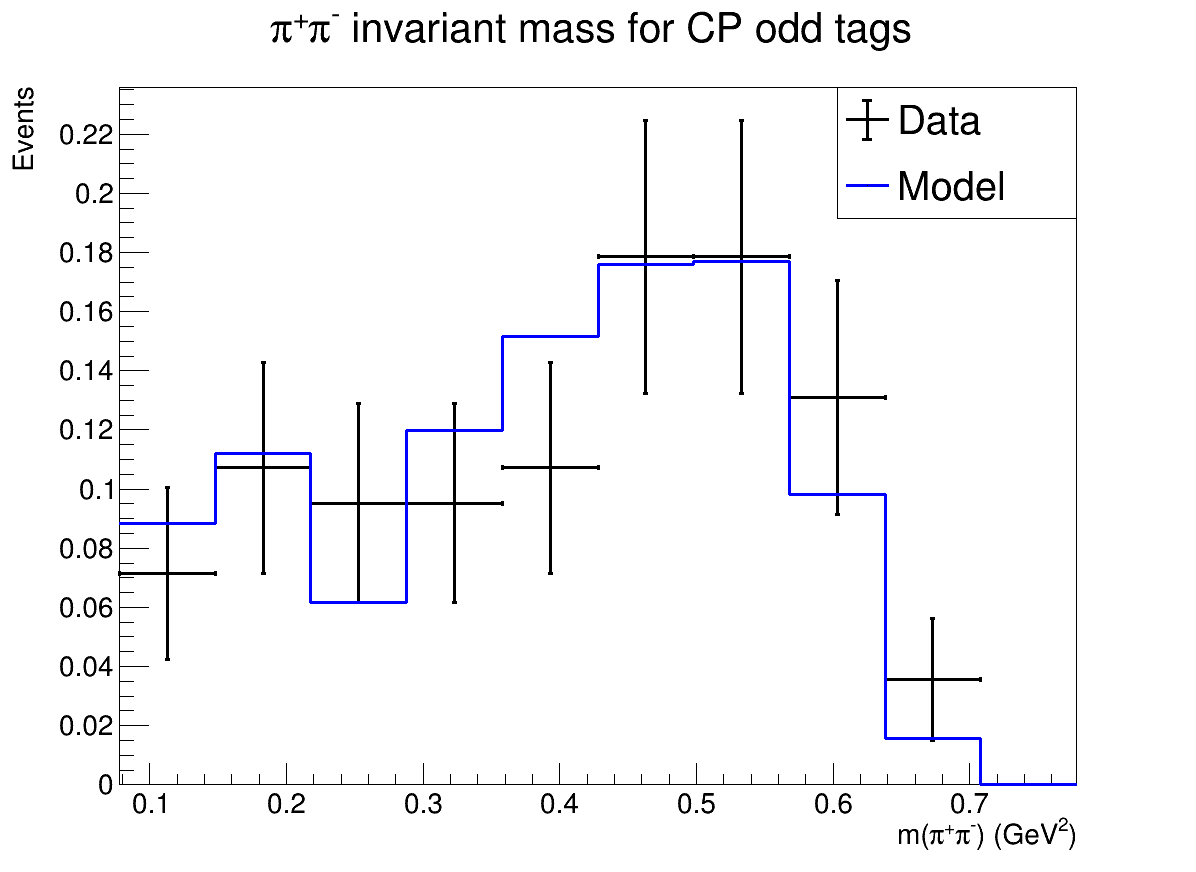
\includegraphics[width = 1.0\textwidth]{Plots/s23_DataModel_CPOddTags.png}
      \caption{Double tags of $KK\pi\pi$ vs CP odd}
    \end{subfigure}
    \caption{$m^2(\pi^+\pi^-)$ in double tags, compared with CP even/odd LHCb models}
  \end{figure}
\end{frame}

\subsection{Current status}

\begin{frame}{Current status}
  \begin{itemize}
    \setlength\itemsep{1.5em}
    \item{Final fit result: $F_+ = \SI{0.73(4)}{}$}
    \begin{itemize}
      \item{First model-independent measurement}
      \item{Compare with model prediction: $F_+ = 0.736$}
      \item{Good news for GLW analyses: Can include $D\to KK\pi\pi$}
    \end{itemize}
    \item{Systematics studies finished}
    \begin{itemize}
      \item{Very small, completely statistics dominated}
    \end{itemize}
    \item{Analysis note (MEMO) written up and reviewed by charm conveners}
    \begin{itemize}
      \item{All three conveners approved last week}
      \item{Next step: Present to BESIII on Friday before entering RC}
    \end{itemize}
  \end{itemize}
\end{frame}
        

\section{Summary}

\begin{frame}{Summary}
  \begin{itemize}
    \setlength\itemsep{1.0em}
    \item{LHCb $B^\pm\to(K^+K^-\pi^+\pi^-)_Dh^\pm$ GGSZ+GLW analysis:}
    \begin{itemize}
      \setlength\itemsep{0.0em}
      \item{Final result of GGSZ part: $\gamma = \SI{103(14)}{}$}
      \item{In RC, currently waiting for further comments}
      \item{$\gamma$($\delta_B^{DK}$) too large(small), still looking for bugs}
    \end{itemize}
    \item{BESIII $D\to K^+K^-\pi^+\pi^-$ strong-phase analysis:}
    \begin{itemize}
      \setlength\itemsep{0.0em}
      \item{First model-independent measurement: $F_+ = \SI{0.73(4)}{}$}
      \item{Analysis required model-dependent efficiency corrections}
      \item{Will present to BESIII on Friday \sout{3rd June} 10th June before entering RC}
    \end{itemize}
    \item{What now?}
    \begin{itemize}
      \item{Currently studying PID performance with TORCH}
      \item{Start at CERN next Monday!}
    \end{itemize}
  \end{itemize}
  \begin{center}
    \huge Thank you!
  \end{center}
\end{frame}

\end{document}
